\documentclass[a4paper,11pt]{book}
%\documentclass[a4paper,twoside,11pt,titlepage]{book}
\usepackage{listings}
\usepackage[utf8]{inputenc}
\usepackage[spanish]{babel}

% \usepackage[style=list, number=none]{glossary} %
%\usepackage{titlesec}
%\usepackage{pailatino}

\decimalpoint
\usepackage{dcolumn}
\newcolumntype{.}{D{.}{\esperiod}{-1}}
\makeatletter
\addto\shorthandsspanish{\let\esperiod\es@period@code}
\makeatother


%\usepackage[chapter]{algorithm}
\RequirePackage{verbatim}
%\RequirePackage[Glenn]{fncychap}
\usepackage{fancyhdr}
\usepackage{graphicx}
\usepackage{afterpage}

\usepackage{subcaption}
\usepackage{rotating}

\usepackage[normalem]{ulem}
\useunder{\uline}{\ul}{}

\usepackage{float}
\usepackage[spanish,onelanguage]{algorithm2e} %for psuedo code

% Math style letters
\usepackage{amsfonts}
\usepackage{amsmath}
\usepackage{amssymb}

\usepackage{longtable}

\usepackage[pdfborder={000},hidelinks]{hyperref} %referencia


%%%%%%%%%%%%%%%%%%%%%%%%%%%%%%%%%%%%%%%%%%%%%%%%%%%%%%%%%%%%%%%%%%%%%%%%%%%%%%%%%%%%%%%%%%%%%%%%%%
%%                                 Para codigo python                                           %%
%%%%%%%%%%%%%%%%%%%%%%%%%%%%%%%%%%%%%%%%%%%%%%%%%%%%%%%%%%%%%%%%%%%%%%%%%%%%%%%%%%%%%%%%%%%%%%%%%%

\usepackage{color}
\usepackage{listings}
\usepackage{setspace}
\definecolor{Code}{rgb}{0,0,0}
\definecolor{Decorators}{rgb}{0.5,0.5,0.5}
\definecolor{Numbers}{rgb}{0.5,0,0}
\definecolor{MatchingBrackets}{rgb}{0.25,0.5,0.5}
\definecolor{Keywords}{rgb}{0,0,1}
\definecolor{self}{rgb}{1,0,0.5}
\definecolor{Strings}{rgb}{0,0.63,0}
\definecolor{Comments}{rgb}{0,0.63,1}
\definecolor{Backquotes}{rgb}{0,0,0}
\definecolor{Classname}{rgb}{1,0,0.5}
\definecolor{FunctionName}{rgb}{0,0,1}
\definecolor{Operators}{rgb}{1,0,0.5}
\definecolor{Background}{rgb}{0.98,0.98,0.98}
\lstdefinelanguage{Python}{
	numbers=left,
	numberstyle=\footnotesize,
	numbersep=1em,
	xleftmargin=1em,
	framextopmargin=2em,
	framexbottommargin=2em,
	showspaces=false,
	showtabs=false,
	showstringspaces=false,
	frame=l,
	tabsize=4,
	% Basic
	basicstyle=\ttfamily\small\setstretch{1},
	backgroundcolor=\color{Background},
	% Comments
	commentstyle=\color{Comments}\sffamily,
	% Strings
	stringstyle=\color{Strings},
	morecomment=[s][\color{Strings}]{"""}{"""},
	morecomment=[s][\color{Strings}]{'''}{'''},
	% keywords
	morekeywords={import,from,class,def,for,while,if,is,in,elif,else,not,and,or,print,break,continue,return,True,False,None,access,as,,del,except,exec,finally,global,import,lambda,pass,print,raise,try,assert},
	keywordstyle={\color{Keywords}\bfseries},
	% additional keywords
	morekeywords={[2]@invariant,pylab,numpy,np,scipy},
	keywordstyle={[2]\color{Decorators}\slshape},
	emph={self},
	emphstyle={\color{self}\slshape},
	%
}

%%%%%%%%%%%%%%%%%%%%%%%%%%%%%%%%%%%%%%%%%%%%%%%%%%%%%%%%%%%%%%%%%%%%%%%%%%%%%%%%%%%%%%%%%%%%%%%%%%

% ********************************************************************
% Re-usable information
% ********************************************************************
%\newcommand{\myTitle}{Biblioteca de algoritmos de detección de anomalías basados en técnicas de ensembles\xspace}
%\newcommand{\myDegree}{Doble grado Ingeniería Informática y Matemáticas\xspace}
%\newcommand{\myName}{Ignacio Aguilera Martos\xspace}
%\newcommand{\myProf}{Francisco Herrera Triguero\xspace}
%%\newcommand{\mySupervisor}{Put name here\xspace}
%\newcommand{\myFaculty}{Escuela Técnica Superior de Ingenierías Informática y de
%Telecomunicación y Facultad de Ciencias\xspace}
%\newcommand{\myFacultyShort}{E.T.S. de Ingenierías Informática y de
%Telecomunicación y Facultad de Ciencias\xspace}
%\newcommand{\myDepartment}{Departamento de Ciencias de la Computación e Inteligencia Artificial\xspace}
%\newcommand{\myUni}{\protect{Universidad de Granada}\xspace}
%\newcommand{\myLocation}{Granada\xspace}
%\newcommand{\myTime}{\today\xspace}
%\newcommand{\myVersion}{Version 0.1\xspace}
%
%
%\hypersetup{
%pdfauthor = {\myName (nacheteam@correo.ugr.es)},
%pdftitle = {\myTitle},
%pdfsubject = {},
%pdfkeywords = {outlier, anomalía, ensemble},
%pdfcreator = {LaTeX},
%pdfproducer = {pdflatex}
%}


%\hyphenation{}


%\usepackage{doxygen/doxygen}
%\usepackage{pdfpages}
\usepackage{url}
\usepackage{colortbl,longtable}
\usepackage[stable]{footmisc}
%\usepackage{index}

%\makeindex
%\usepackage[style=long, cols=2,border=plain,toc=true,number=none]{glossary}
% \makeglossary

% Definición de comandos que me son tiles:
%\renewcommand{\indexname}{Índice alfabético}
%\renewcommand{\glossaryname}{Glosario}

\pagestyle{fancy}
\fancyhf{}
\fancyhead[LO]{\leftmark}
\fancyhead[RE]{\rightmark}
\fancyhead[RO,LE]{\textbf{\thepage}}
\renewcommand{\chaptermark}[1]{\markboth{\textbf{#1}}{}}
\renewcommand{\sectionmark}[1]{\markright{\textbf{\thesection. #1}}}

\setlength{\headheight}{1.5\headheight}

\newcommand{\HRule}{\rule{\linewidth}{0.5mm}}
%Definimos los tipos teorema, ejemplo y definición podremos usar estos tipos
%simplemente poniendo \begin{teorema} \end{teorema} ...
\newtheorem{teorema}{Teorema}[chapter]
\newtheorem{proposicion}{Proposición}[chapter]
\newtheorem{propiedad}{Propiedad}[chapter]
\newtheorem{lema}{Lema}[chapter]
\newtheorem{demostracion}{Demostración}[chapter]
\newtheorem{propiedades}{Propiedades}[chapter]
\newtheorem{ejemplo}{Ejemplo}[chapter]
\newtheorem{definicion}{Definición}[chapter]

\newcommand*{\QEDA}{\hfill\ensuremath{\blacksquare}}%
\newcommand*{\QEDB}{\hfill\ensuremath{\square}}%

\definecolor{gray97}{gray}{.97}
\definecolor{gray75}{gray}{.75}
\definecolor{gray45}{gray}{.45}
\definecolor{gray30}{gray}{.94}

\lstset{ frame=Ltb,
     framerule=0.5pt,
     aboveskip=0.5cm,
     framextopmargin=3pt,
     framexbottommargin=3pt,
     framexleftmargin=0.1cm,
     framesep=0pt,
     rulesep=.4pt,
     backgroundcolor=\color{gray97},
     rulesepcolor=\color{black},
     %
     stringstyle=\ttfamily,
     showstringspaces = false,
     basicstyle=\scriptsize\ttfamily,
     commentstyle=\color{gray45},
     keywordstyle=\bfseries,
     %
     numbers=left,
     numbersep=6pt,
     numberstyle=\tiny,
     numberfirstline = false,
     breaklines=true,
   }
 
% minimizar fragmentado de listados
\lstnewenvironment{listing}[1][]
   {\lstset{#1}\pagebreak[0]}{\pagebreak[0]}

\lstdefinestyle{CodigoC}
   {
	basicstyle=\scriptsize,
	frame=single,
	language=C,
	numbers=left
   }
\lstdefinestyle{CodigoC++}
   {
	basicstyle=\small,
	frame=single,
	backgroundcolor=\color{gray30},
	language=C++,
	numbers=left
   }

 
\lstdefinestyle{Consola}
   {basicstyle=\scriptsize\bf\ttfamily,
    backgroundcolor=\color{gray30},
    frame=single,
    numbers=none
   }


\newcommand{\bigrule}{\titlerule[0.5mm]}


%Para conseguir que en las páginas en blanco no ponga cabecerass
\makeatletter
\def\clearpage{%
  \ifvmode
    \ifnum \@dbltopnum =\m@ne
      \ifdim \pagetotal <\topskip
        \hbox{}
      \fi
    \fi
  \fi
  \newpage
  \thispagestyle{empty}
  \write\m@ne{}
  \vbox{}
  \penalty -\@Mi
}
\makeatother

\usepackage{pdfpages}
\begin{document}
\setlength{\parskip}{10pt}

\begin{titlepage}
 
 
\newlength{\centeroffset}
\setlength{\centeroffset}{-0.5\oddsidemargin}
\addtolength{\centeroffset}{0.5\evensidemargin}
\thispagestyle{empty}

\noindent\hspace*{\centeroffset}\begin{minipage}{\textwidth}

\centering

\includegraphics[width=0.9\textwidth]{imagenes/logos/logo_ugr.jpg}\\[1.4cm]

\textsc{ \Large TRABAJO FIN DE MÁSTER\\[0.2cm]}
\textsc{ Máster Oficial en Ciencia de Datos e Ingeniería de Computadores}\\[1cm]
% Upper part of the page
% 
% Title
{\Huge\bfseries Detección de Anomalías en Series Temporales basada en técnicas Deep Learning\\
}
\noindent\rule[-1ex]{\textwidth}{3pt}\\[3.5ex]
{\large\bfseries Biblioteca de algoritmos}
\end{minipage}

\vspace{2.5cm}
\noindent\hspace*{\centeroffset}\begin{minipage}{\textwidth}
\centering

\textbf{Autor}\\ {Ignacio Aguilera Martos}\\[2.5ex]
\textbf{Director}\\
{Francisco Herrera Triguero}\\[2cm]

\includegraphics[width=0.3\textwidth]{imagenes/logos/etsiit_logo.png}\\[0.1cm]
\textsc{Escuela Técnica Superior de Ingenierías Informática y de Telecomunicación}\\

\includegraphics[width=0.2\textwidth]{imagenes/logos/ciencias.png}\\[0.1cm]
\textsc{Facultad de Ciencias}\\
\textsc{---}\\
Granada, 10 de Septiembre de 2020
\end{minipage}
%\addtolength{\textwidth}{\centeroffset}
%\vspace{\stretch{2}}
\end{titlepage}



\chapter*{}
%\thispagestyle{empty}
%\cleardoublepage

%\thispagestyle{empty}

\begin{titlepage}
 
 
\setlength{\centeroffset}{-0.5\oddsidemargin}
\addtolength{\centeroffset}{0.5\evensidemargin}
\thispagestyle{empty}

\noindent\hspace*{\centeroffset}\begin{minipage}{\textwidth}

\centering
%
\includegraphics[width=0.9\textwidth]{imagenes/logo_ugr.jpg}\\[1.4cm]

%\textsc{ \Large PROYECTO FIN DE CARRERA\\[0.2cm]}
%\textsc{ INGENIERÍA EN INFORMÁTICA}\\[1cm]
% Upper part of the page
% 

 \vspace{3.3cm}

%si el proyecto tiene logo poner aquí
%
\includegraphics{imagenes/logo.png} 
% \vspace{0.5cm}

% Title

{\Huge\bfseries Detección de Anomalías en Series Temporales basada en técnicas Deep Learning\\
}
\noindent\rule[-1ex]{\textwidth}{3pt}\\[3.5ex]
{\large\bfseries Biblioteca de algoritmos\\[4cm]}
\end{minipage}

\vspace{2.5cm}
\noindent\hspace*{\centeroffset}\begin{minipage}{\textwidth}
\centering

\textbf{Autor}\\ {Ignacio Aguilera Martos}\\[2.5ex]
\textbf{Directores}\\
{Francisco Herrera Triguero}\\[2cm]
%
\includegraphics[width=0.15\textwidth]{imagenes/tstc.png}\\[0.1cm]
%\textsc{Departamento de Teoría de la Señal, Telemática y Comunicaciones}\\
%\textsc{---}\\
%Granada, mes de 201
\end{minipage}
%\addtolength{\textwidth}{\centeroffset}
\vspace{\stretch{2}}

 
\end{titlepage}






\cleardoublepage
\thispagestyle{empty}

\begin{center}
{\large\bfseries Detección de Anomalías en Series Temporales basada en técnicas Deep Learning: Biblioteca de algoritmos}\\
\end{center}
\begin{center}
Ignacio Aguilera Martos\\
\end{center}

%\vspace{0.7cm}
\noindent{\textbf{Palabras clave}: % RELLENAR CON LAS PALABRAS CLAVE EN ESPAÑOL
			}\\

\vspace{0.7cm}
\noindent{\textbf{Resumen}}\\

% RELLENAR CON EL ABSTRACT EN ESPAÑOL

\cleardoublepage


\thispagestyle{empty}


\begin{center}
{\large\bfseries Outlier Detection in Time Series using Deep Learning: Library implementation}\\
\end{center}
\begin{center}
Ignacio Aguilera Martos\\
\end{center}

%\vspace{0.7cm}
\noindent{\textbf{Keywords}: % RELLENAR CON LAS PALABRAS CLAVE EN INGLES
			}\\

\vspace{0.7cm}
\noindent{\textbf{Abstract}}\\

% RELLENAR CON EL ABSTRACT EN INGLES

\chapter*{Agradecimientos}
\thispagestyle{empty}

% RELLENAR CON LOS AGRADECIMIENTOS EN ESPAÑOL
\frontmatter
\tableofcontents
%\listoffigures
%\listoftables
%
\mainmatter

\chapter{Introducción}
\label{chapter:introduccion}
\markboth{Introducción}{}
\pagenumbering{arabic}
\setcounter{page}{1}

Antes de comenzar con el desarrollo en sí del estudio acometido en este trabajo, vamos a contextualizar el mismo y vamos a establecer un marco de trabajo teórico previo a la experimentación, que nos otorgará de rigurosidad para la parte práctica del mismo.

El estudio realizado en este trabajo versa sobre la aplicación de estructuras de Aprendizaje Profundo (Deep Learning) para obtención y detección de anomalías, en concreto, en series temporales. Dentro de este trabajo se van a desarrollar las técnicas conocidas como Autoencoders y Redes Neuronales para predicción de series temporales.

Lo primero que atacaremos en este estudio es la definición de anomalía, para luego pasar a una introducción teórica de Estadística Multivariante y Machine Learning en general. Estas dos secciones nos van a aportar el rigor que necesitamos para adentrarnos teóricamente dentro del Deep Learning y entender los fundamentos de las arquitecturas de redes neuronales que aplicaremos en la práctica.

Tras esto se realizará una descripción de la experimentación realizada, los datos que se emplearán en dicha experimentación y los resultados de la misma. 

%%%%%%%%%%%%%%%%%%%%%%%%%%%%%%%%%%%%%%%%%%%%%%%%%

\section{Contextualización}

Lo primero que debemos de hacer antes de empezar, es establecer el problema u objetivo a resolver de este estudio. Para ello vamos a hacer una breve introducción a los datos (o al problema propuesto que es lo mismo en este ámbito) y a explicar por qué precisamos de un trabajo arduo y prolongado, es decir, por qué no es un problema trivial.

\subsection{Definición del problema}

El ámbito de trabajo va a ser el de las series temporales, pues el conjunto de datos que nos define el problema es una serie temporal. Esta serie temporal mide la sensórica de una máquina de la empresa ArcelorMittal, que no podemos especificar por motivos de privacidad. En este sentido tenemos 106 variables de tipo numérico con las que vamos a trabajar y 468 días de datos con una granularidad de una medida por segundo. Esto hace que el volumen de datos del que disponemos sea inmenso, haciendo que tenga sentido el uso del Deep Learning por la enorme cantidad de datos de entrenamiento de los que vamos a disponer.

Como hemos comentado los datos son medidas de sensores de una cierta máquina. Esta máquina experimenta errores graves de vez en cuando, que hacen que se deba detener completamente para labores de mantenimiento. Nuestro objetivo es ser capaces de detectar estas labores de mantenimiento mediante técnicas de detección de anomalías. El principio subyacente es sencillo: esperamos un comportamiento normal de la máquina en la mayoría del tiempo salvo cuando haya necesidad de un mantenimiento, momento en el cual la sensórica arrojará medidas alteradas que nos den pie a pensar en un posible fallo.

Este tipo de problemas son conocidos como mantenimiento predictivo, pues lo que pretenden precisamente es anticipar la necesidad de dichas labores.

Con esto dicho nuestro objetivo será tomar los datos de entrada (la sensórica) para nuestros modelos Deep Learning y, de alguna manera, saber diferenciar lo que son datos normales y datos anómalos.

\section{Contenido básico y fuentes}

% REVISAR CUANDO TERMINE EL CONTENIDO %

El trabajo contiene una primera sección en la que se incluye una introducción de Aprendizaje Automático orientado específicamente a nuestro problema. Para ello primero se hace una contextualización del concepto de aprendizaje así como los principios inductivos que guían el mismo hacia un buen resultado como por ejemplo el ERM o minimización del error empírico. Se aportan también algunas reflexiones y conceptos en cuanto a la aproximación de funciones, que no es más que el objetivo del aprendizaje automático. 

Todos estos conocimientos están basados en la teoría estadística de Vapnik y Chervonenkis que es brevemente repasada y en la que se dan cotas sobre el aprendizaje y su rendimiento. Esta introducción ha sido escrita basándose en tres libros: Learning from Data de Yaser Abu-Mostafa \cite{yaser_learning_2012}, Learning from Data de Cherkassky y Mulier \cite{cherkassky_learning_2007}  y Outlier Ensembles de Aggarwal y Sathe \cite{aggarwal_outlier_2017}.

Este marco nos dirige hacia la primera definición del concepto de anomalía que está basada en distancias y rangos intercuartil que se describen en el libro Outlier Analysis \cite{aggarwal_outlier_2017-1}. Además se introduce el tipo de datos que vamos a encontrar en el marco del estudio: las series temporales.

Para dar una definición alternativa y una buena base teórica para los modelos debemos hacer una breve introducción estadística. En esta introducción se define un vector aleatorio así como su función de densidad, su función característica y su función de distribución. Se refieren los conceptos de independencia y probabilidad y esperanza condicionada. Por último y aprovechando este contexto se enuncian y demuestran algunas desigualdades y fórmulas famosas. Este contenido viene dado por los apuntes de la asignatura Estadística Multivariante del grado en Matemáticas, los apuntes de la asignatura Procesos Estocásticos del grado en Matemáticas y el libro Probability Theory de M. Loève \cite{m._loeve_probability_1977}.

Tras esto puede ser introducido el concepto probabilístico y basado en densidad de una anomalía. Este concepto viene apoyado en el paper \cite{fabian_keller_hics:_2012} que describe el algoritmo HICS.

Tras este marco teórico de aprendizaje, estadística multivariante y definiciones de anomalías introducimos los conocimientos necesarios de Deep Learning para el desarrollo y entendimiento de los modelos no supervisados implementados. Esta sección hace una revisión de cómo funcionan las redes neuronales, distintos tipos de capas empleados en las arquitecturas implementadas y algunas arquitecturas con mayor fundamentación académica como los Autoencoder. Esta sección se apoya en el libro Deep Learning de Goodfellow, Bengio y Courville \cite{goodfellow_deep_2016}, el libro Deep Learning with Tensorflow de Zaccone, Karim y Menshawy \cite{giancarlo_deep_2017} y la revisión sobre modelos Autoencoder de D. Charte, F. Charte, García, Mª J. del Jesús y F. Herrera \cite{david_practical_2018}.

La siguiente sección analiza y explica los modelos implementados con su código propio. Esta sección se apoya en varios artículos como \cite{lih_oh_automated_2018} o \cite{david_practical_2018} para obtener las arquitecturas empleadas y aplicarlas al ámbito no supervisado que necesitamos.

La siguiente sección explica cómo se integran los algoritmos de detección de anomalías para poder ser empleados para detectar los mantenimientos y cómo obtenemos etiquetas de los datos.

Tras esto se exponen los resultados obtenidos así como la metodología de la experimentación para finalizar con las conclusiones y trabajo futuro derivados del estudio.

\section{Objetivos}

Por todo lo descrito anteriormente el trabajo tiene los siguientes objetivos claros:

\begin{itemize}
	\item Desarrollar un marco teórico sobre el Machine Learning.
	\item Desarrollar un marco teórico sobre el Deep Learning.
	\item Estudiar el estado del arte de los algoritmos de detección de anomalías que emplean Deep Learning.
	\item Estudiar la teoría estadística que rodea el Machine Learning y el Deep Learning.
	\item Entender los fundamentos teóricos y el funcionamiento de los modelos implementados.
	\item Desarrollar una implementación de los modelos.
	\item Obtener una comparativa entre los modelos clásicos y los Deep Learning.
\end{itemize}

Todos estos objetivos han sido alcanzados en el desarrollo de este estudio, obteniendo conclusiones de calidad y líneas de trabajo futuro que se aplicarán a la continuidad del proyecto.
%
\part{Machine Learning, Deep Learning y el concepto de anomalía}
\label{part:machine_learning_deep_learning_anomalia}

\chapter{Concepto de Anomalía y Series Temporales}
\label{chapter:anomalia}

\section{Concepto de Anomalía}

Debemos de tener en cuenta que el concepto de anomalía no es algo fácil de definir. Tanto es así que, por ligeros cambios o matices en la definición, podemos estar cayendo en un concepto completamente distinto.

Antes de comenzar debemos aclarar el objetivo que vamos persiguiendo, es decir, el concepto de anomalía que nos va a interesar. Podemos encontrar muchas definiciones de anomalías, pero en nuestro caso nos vamos a centrar en la dada por Carreño, Inza y Lozano en \cite{ander_analyzing_2019}.

Según estos autores podemos definir el contexto de la detección de anomalías en 4 subtipos: eventos raros, anomalías, novedades y outliers. 

En primer lugar, tenemos los eventos raros. Tenemos un problema en el que hay un tipo de datos que aparecen con muy poca frecuencia en el contexto de las series temporales y queremos detectar dicho tipo de eventos. Estamos en una perspectiva supervisada, por lo que esto no es más que un problema de clasificación altamente desbalanceado en el contexto de las series temporales. En este escenario el problema se resuelve aplicando distintas técnicas que favorezcan que los clasificadores aprendan bien esta clase rara y se detecte. Claramente no es nuestro caso pues no disponemos de etiquetas claras y no es un problema de clasificación.

En segundo lugar tenemos las anomalías. Según Carreño, las anomalías están enmarcadas en conjuntos de datos estáticos. Este simple hecho ya saca el subtipo de nuestro marco de trabajo, pero aún así es bueno ver su definición. Las anomalías son, para Carreño et al., un problema de clasificación altamente desbalanceado en el contexto de datos estáticos. Esto es análogo al caso anterior, salvando el paso de datos estáticos a dinámicos. Claramente no es nuestro caso pues el problema no es de clasificación ni tenemos etiquetas claras ni son datos estáticos de los que disponemos.

En tercer lugar tenemos las novedades. Este apartado puede ser aplicado tanto a datos estáticos como a datos dinámicos. En los dos casos anteriores tenemos problemas de clasificación, pero disponemos de las etiquetas y de ejemplos de todas las clases para la fase de entrenamiento. En las novedades tenemos datos normales de una sola clase en la fase de entrenamiento, por lo que en el momento de entrenar tendremos que definir las fronteras de la única clase que tenemos. El objetivo en este problema es detectar la novedad, es decir, los nuevos ejemplos que no cuadran dentro de la frontera de decisión de la única clase que tenemos en la fase de entrenamiento en el problema. De nuevo esto no es nuestro caso, porque no tenemos etiquetas de los datos normales y por tanto no podemos definir claramente ese marco de trabajo ``one class''.

Por último tenemos los outliers. Este término no es de fácil traducción al español, por lo que es preferible dejar el original en inglés. Este punto engloba la clasificación no supervisada, es decir, tenemos ciertas nociones del conjunto de datos pero ninguna etiqueta precisa y aun así queremos saber qué datos son normales y cuáles anómalos basándonos en alguna técnica que no emplee más que los propios datos sin etiquetar. Este es nuestro marco de trabajo, pues no disponemos de etiquetas claras ni ``ground truth'', oráculo o verdad absoluta a la que recurrir para aprender de ella. Tenemos que elaborar un sistema capaz de detectar los mantenimientos de nuestra máquina sin poder aprender a priori lo que es normal y lo que es anómalo.

Dentro de este esquema de posibilidades ya hemos localizado la que más se acerca al objetivo que queremos cumplir. Como hemos podido ver, es la única opción completamente no supervisada que Carreño contempla en el artículo, lo que nos deja con el escenario más complejo de todos. 

Pensemos un momento todas las posibles definiciones de anomalías que tenemos mediante varios ejemplos.

\begin{figure}[H]
	\centering
	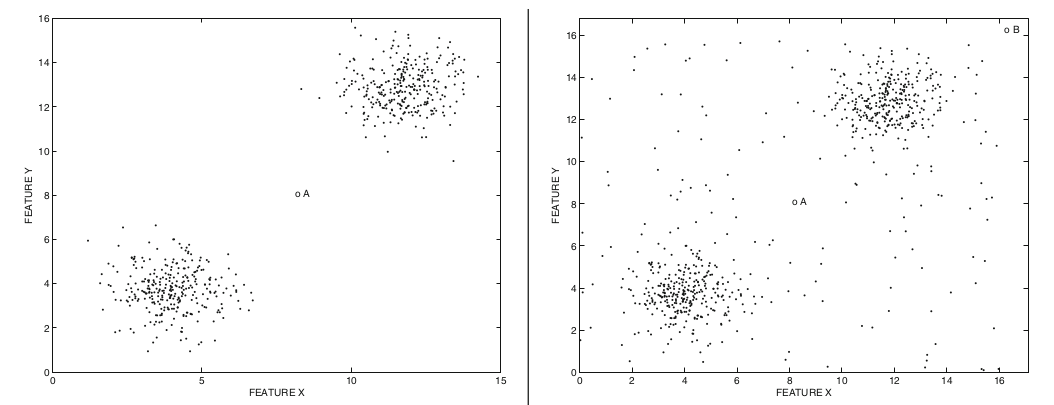
\includegraphics[scale=0.35]{imagenes/ejemplo1_anomalia.png}
	\caption{Ejemplo sin ruido y con ruido de una anomalía. \cite[p21]{aggarwal_outlier_2017}}
	\label{img:ejemplo1-anomalia}
\end{figure}

Como podemos ver, el caso de la izquierda es relativamente fácil de detectar, por ejemplo con un algoritmo de clústering. El ejemplo de la derecha es muchísimo más complejo. En el ejemplo tenemos identificado el mismo punto como anomalía, pero ahora está rodeado de ruido que hace muy complicado detectarlo. Además surge la pregunta de cuándo tenemos ruido y cuándo son puntos anómalos ya que la diferencia en algunos casos es inapreciable.

Para todas estas cuestiones no hay una respuesta que siempre sea la adecuada, pues dependen del contexto en el que estemos y de lo que queramos detectar y hacer con las anomalías. Los algoritmos de detección de anomalías, al no ser fácil la tarea de clasificación por ser no supervisado, nos suelen arrojar un número que puntúa cada instancia. Cuanto mayor sea el número asignado a una instancia mayor es su grado de anomalía. Este sistema nos permite asignar algún tipo de regla que detecte los puntos más anómalos y deje fuera los puntos de los que no estemos seguros. Por tanto, un algoritmo de detección de anomalías por si solo para este problema no es de utilidad. Hay que acompañarlo de un sistema que decida sobre los scores qué puntos son anómalos y cuales no, además de que en nuestro problema no tenemos datos estáticos, si no series temporales, por lo que debemos también dotar de esa temporalidad a las anomalías.

Todos estos aspectos los discutiremos más a fondo cuando nos acerquemos a la sección de experimentación, donde podremos ver mejor la forma final de detectar anomalías y mantenimientos en nuestro caso.

\section{Series Temporales}

Ya hemos comentado que vamos a trabajar con series temporales, por lo que antes de empezar cabe definir formalmente lo que consideramos una serie temporal.

Una serie temporal podemos definirla como un par $(t,x)\in \mathbb{R}\times \mathbb{R}$ donde $t$ es un sello temporal, es decir, una cuantificación numérica para el tiempo desde un punto de referencia y $x$ es un valor numérico asociado al valor temporal. De esta forma lo que tenemos son valores numéricos para cada valor temporal.

Si extendemos este concepto podemos definirlo como $(t,x)\in \mathbb{R}\times \mathbb{R}^n$ donde $n$ es la dimensionalidad de la serie temporal, es decir, ahora no toma valores reales si no vectores de valores reales.

Las series temporales se pueden dividir en varias componentes. Esta división tiene la intención de poder entender mejor el comportamiento de la serie, tanto para su estudio como el posterior modelado y predicción si nos interesase.

Las componentes que podemos extraer de una serie temporal son:

\begin{itemize}
	\item Tendencia: nos indica la componente que se mantiene estable a lo largo de toda la serie temporal, por ejemplo podemos tener tendencias crecientes, decrecientes o no tener tendencia en nuestra serie.
	\item Componente estacional: es la componente cíclica que se repite con periodos menores a un año, por ejemplo puede ser por estaciones, meses, semanas u otra fracción de tiempo significativa para el problema.
	\item Componente cíclica: es la componente que recoge los fenómenos periódicos de frecuencia mayor a un año, normalmente de periodo irregular influida por movimientos a menudo dependientes de la tendencia.
	\item Componente residual: es la componente que depende del ambiente del sistema. No tiene ningún tipo de regularidad y podemos decir que depende de las anomalías que se presenten en la serie de forma más común o frecuente.
	\item Componente accidental: esta componente recoge las variaciones que se producen por fenómenos muy raros y aislados.
\end{itemize}

Podemos poner un ejemplo para ilustrar las componentes de una serie. Por ejemplo si tenemos una serie temporal con las temperatura de la tierra actualmente podemos apreciar una tendencia creciente por el cambio climático, por lo que la componente de la tendencia sería creciente. Tenemos una componente estacional que podemos apreciar por las estaciones del año, momentos en los cuales las temperaturas bajan y suben siempre de la misma forma o muy similar. La componente cíclica puede ser por ejemplo las edades de la Tierra, momentos en los cuales las temperaturas bajan y suben dependiendo de las glaciaciones y la flora y fauna de la Tierra. En la componente residual podemos tener por ejemplo fenómenos como tormentas, inundaciones o fenómenos producidos por el hombre. En la componente accidental tendríamos fenómenos mucho más súbitos y repentinos, por ejemplo podríamos poner en esta componente la caída de un meteorito, fenómeno que raramente puede producirse más de una vez o dos.

Visto esto, ya tenemos una idea de lo que vamos a ir buscando y el tipo de datos con los que vamos a tratar. En nuestra serie temporal nosotros nos vamos a preocupar por la componente residual y la accidental, ya que son las componentes en las que se esconden los fenómenos que no son modelables y por tanto escapan al comportamiento normal de las variables.
%
%\chapter{Concepto de anomalía}
\label{chapter:anomalia}

En esta sección vamos a estudiar la idea de anomalía, fundamentalmente propuesta en el libro Outlier Analysis \cite{aggarwal_outlier_2017-1}.

\section{Contextualización}

Ya hemos discutido previamente una idea intuitiva del concepto de anomalía. Un dato decimos que es anómalo cuando se distancia del resto de los datos lo suficiente como para no tener características comunes con ellos.

Este hecho puede ser por distintos motivos. Puede que la anomalía venga del hecho de que se está produciendo un evento en nuestros experimentos que no sea nada frecuente. Por ejemplo podemos estar midiendo datos meteorológicos y que en un momento dado se den una serie de fenómenos que no sea frecuente ver juntos, o incluso que no se hayan visto nunca ocurrir simultáneamente. Otra forma de tener una anomalía en nuestro conjunto de datos pudiera ser errores de medición. Por ejemplo si seguimos con este símil de los datos meteorológicos imaginemos que nuestra estación dispone de un termómetro. Este sensor se ha roto y empieza a marcar datos superiores a 100 $C^\circ$, claramente son datos muy desviados de las temperaturas normales con lo que no tendrían relación con el resto y presentaría una desviación muy importante con respecto al resto de los datos.

\section{Criterios}

Esta idea intuitiva que estamos dando de anomalía no refleja todos los posibles escenarios. Los ejemplos que estamos dando suponen una desviación muy grande de los datos normales, tanto que no se pueden comparar con el resto porque difieren mucho numéricamente. Vamos a plantear un escenario para dar una mejor forma al concepto de anomalía. Pensemos en una serie de datos muy agrupados en dos clústeres por ejemplo:

\begin{figure}[H]
	\centering
	\includegraphics[scale=0.5]{imagenes/clusters}
	\label{clusters}
	\caption{Clústeres alejados}
\end{figure}

Como podemos comprobar que tenemos dos clústeres no sólo alejados entre sí, si no con los elementos muy concentrados para poner un caso extremo. Ahora no vamos a proponer un valor que se aleje de los dos clústeres, si no uno que esté a medio camino entre los dos:

\begin{figure}[H]
	\centering
	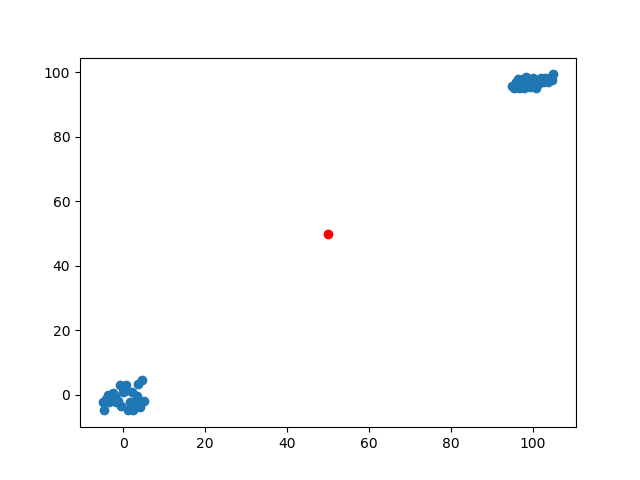
\includegraphics[scale=0.5]{imagenes/outlier_cluster}
	\label{outlier_clusters}
	\caption{Clústeres alejados con una anomalía en rojo}
\end{figure}

Si los datos del clúster de abajo a la izquierda fueran datos de temperatura con valores entorno a 0 y los de arriba a la derecha fueran de datos de temperatura entorno a 100 grados nuestro datos anómalo tendría una temperatura de unos 50 grados. Esta temperatura no se aleja radicalmente de los valores normales, es decir, no son -1000 grados ni 1000 grados. Aún así estamos describiendo una situación anómala.

No podemos dar una definición formal o que podamos decir que abarca todos los casos para definir lo que es una anomalía, aún así vamos a intentar dar dos puntos de vista: uno basado en distancias y otro en probabilidades.

El criterio más usado en la definición o detección de anomalías es el llamado ``Tukey's Fences''. Para introducirlo vamos a ver su definición en una única dimensión para luego extender el concepto. Pensemos en un conjunto de datos 1-D. Sobre sus valores podemos calcular los cuartiles $Q_1 , Q_2 $ y $Q_3$. Un valor anómalo es aquel que no cae dentro del intervalo $[Q_1 - k(Q_3 - Q_1), Q_3 + k(Q_3 - Q_1)]$ donde $k$ es una constante. El valor propuesto para $k$ por Tukey fue de $k=1.5$ aunque algunos autores más restrictivos proponen $k=3$.

Este criterio puede ser extendido al caso de mayor dimensionalidad si realizamos este mismo test sobre todos los valores de todas las características y comprobar si alguno o todos se salen del rango en función de cómo de restrictivo queremos que sea el criterio.

Esta extensión es muy vaga, por lo que se propone un criterio un poco más fijado. Imaginemos los datos agrupados por clústeres, entonces podemos fijar un centroide de dicho clúster. Sobre cada clúster podemos medir cuál es la mayor distancia dentro del clúster de los datos al centroide. Podemos extender el criterio de Tukey diciendo que un dato anómalo es aquel que se distancia más de $1.5$ veces de la mayor distancia dentro del clúster al centroide.

Esta generalización ya si abarca el ejemplo que hemos propuesto. Al estar muy apiñados los datos entorno al centroide la mayor distancia dentro del clúster es muy pequeña, de hecho en el ejemplo construido es menor que 5. Por tanto el dato $(50,50)$ está alejado más de $1.5 \cdot 5 = 7.5$ unidades del centroide y por tanto lo podemos considerar una anomalía.

\section{Qué hacer con las anomalías}

Estamos estudiando cómo podemos detectar anomalías pero una vez que las hayamos detectado en nuestros conjuntos de datos en un problema real, ¿qué debemos hacer con ellas? Este problema es algo muy general, puede que estemos seguros en nuestro caso de que las anomalías se han debido a un problema de medición porque nuestros instrumentos estaban rotos y por tanto deberíamos descartarlos. Puede que sean datos reales pero estén tan separados del resto que debamos estudiarlos de forma separada. Vamos a dar unas cuantas alternativas a lo que podemos hacer una vez que hemos detectados las anomalías dentro de nuestro conjunto de datos:

\begin{itemize}
	\item Dejarlos: puede que nuestro conjunto de datos tenga un número de datos muy elevado y por tanto aparezcan en él anomalías. Estas anomalías no deben ser eliminadas, es más debemos escoger modelos que aprendan o utilicen los datos teniendo en cuenta estas anomalías y siendo robustos ante su aparición.
	\item Exclusión: una opción es eliminar directamente las anomalías. Esto en general no está justificado y de hecho no se recomienda pues perdemos riqueza del conjunto de datos al eliminar instancias del mismo. Aún así, si decidimos eliminar los datos tenemos dos formas de hacerlo. Podemos eliminarlos directamente y prescindir de esos datos o podemos sustituirlos por datos cercanos que no sean anómalos.
	\item Estudiarlos por separado: puede que tengamos un número suficientemente elevado de las mismas y que enseñen algunos patrones o tengan explicación en nuestro ejemplo del mundo real. En este caso quizás deberíamos considerarlas y estudiarlas a parte para darles un sentido y emplear el conocimiento que les subyace.
\end{itemize}
%
%\part{Introducción de Estadística Multivariante y concepto probabilístico de anomalía}
\label{part:multivariante_anomalia2}

Para poder proseguir en el estudio debemos hacer un repaso breve de conceptos de estadística multivariante. El contenido de esta sección se ha sacado básicamente de apuntes de la asignatura Estadística Multivariante del grado en Matemáticas, los apuntes de la asignatura Procesos Estocásticos del grado en Matemáticas y el libro Probability Theory de M. Loève \cite{m._loeve_probability_1977}.

\chapter{Introducción de Estadística Multivariante}
\label{chapter:estadistica_multivariante}

Vamos a dar otra definición de anomalía que no coincide con la que hemos visto basada en distancias, pero antes de dar esa definición debemos hacer un breve repaso de estadística multivariante y probabilidad para poder comprender y enmarcar dicha definición.

\section{Introducción}

En primer lugar vamos a describir conceptos básicos sobre los que poder construir los conceptos que necesitamos para la definición de anomalía basada en probabilidades.

En primer lugar vamos a definir el concepto de variable aleatoria.

\begin{definicion}
	Una variable aleatoria es una función $X:\Omega \rightarrow E$ que parte de un espacio de probabilidad $(\Omega , \mathcal{F}, \mathcal{P})$ y llega a un espacio medible $(E, \mathcal{B})$, donde $X$ además es una función medible.
\end{definicion}

Normalmente ya sabemos que $E\subseteq \mathbb{R}$ y además cabe recordar que $\mathcal{F}$ es una $\sigma$-álgebra. Además cabe recordar la definición de función medible:

\begin{definicion}
	Decimos que una función $X: (\Omega , \mathcal{F}, \mathcal{P}) \rightarrow (E, \mathcal{B})$ es medible si $X^{-1}(B)\subset \mathcal{F}$, $\forall B \in \mathcal{B}$.
\end{definicion}

Esta definición puede extenderse al caso vectorial, introduciendo con esto la noción de vector aleatorio:

\begin{definicion}
	Un vector aleatorio $\underline{X} = (X_1 , ... , X_p)$ es una aplicación medible $\underline{X}: (\Omega , \mathcal{F}, \mathcal{P})\rightarrow (E, \mathcal{B}^p)$ donde $E\subseteq \mathbb{R}^p$.
\end{definicion}

Se puede demostrar además la caracterización:

\begin{proposicion}
	Un vector $\underline{X} = (X_1, ..., X_p)$ es un vector aleatorio si y sólo si $X_i : (\Omega , \mathcal{F}, \mathcal{P}) \rightarrow (\mathbb{R}, \mathcal{B})$ es una función medible.
\end{proposicion}

Con este vector aleatorio podemos estudiar o definir la distribución de probabilidad del mismo sobre $( \mathbb{R}^p , \mathcal{B}^p )$ $P_{\underline{X}}$ como:

$$P_{\underline{X}} [B]:= P[\underline{X}^{-1}(B)] \ \forall B\in \mathcal{B}$$

con lo que el espacio $(\mathbb{R}^p , \mathcal{B}^p , P_{\underline{X}})$ es un espacio de probabilidad o probabilístico.

Sobre los conocimientos de la definición de la función de distribución univariante podemos hacer una definición análoga para el caso multivariante.

\begin{definicion}
	Se define la función de distribución asociada a la probabilidad inducida como:
	
	$$F_{\underline{X}} (\underline{x}) = P_{\underline{X}} [X_1 \leq x_1 , ... , X_p \leq x_p] \ , \ \forall \underline{x} = (x_1 , ... , x_p) \in \mathbb{R}^p$$
\end{definicion}

De igual forma podemos caracterizar la función de densidad como aquella $f_{\underline{X}}$ que, de existir, cumple que:

$$F_{\underline{X}} (\underline{x}) = \int_{- \infty}^{x_1} \int_{-\infty}^{x_2} ... \int_{-\infty}^{x_p} f_{\underline{X}}(u_1 , ... , u_p) du_1 ... du_p$$

Otra forma de determinar de forma única la distribución de un vector aleatorio es mediante la función característica, lo que nos va a dar además una caracterización de la independencia que introduciremos seguidamente.

\begin{definicion}
	Dado un vector aleatorio $X = (X_1 , ... , X_p)$ se define la función característica como $\Phi_{\underline{X}} (\underline{t}) = E[e^{i\underline{t}X}]$ con $\underline{t} = (t_1 , ... , t_p)\in \mathbb{R}^p$ donde la función $E[\cdot]$ denota la esperanza, por lo que:
	$$\Phi_{\underline{X}} (\underline{t}) = \int_{\mathbb{R}^p} e^{i\underline{t} \underline{X}} P_{\underline{X}}(d\underline{x})$$
\end{definicion}

Con esto ya podemos introducir el concepto de independencia en varias variables. 

\subsection{Independencia}

\begin{definicion}
	Dados dos vectores aleatorios $\underline{X} = (X_1 , ... , X_p)$, $\underline{Y} = (Y_1 , ... , Y_p)$ se dice que son independientes si:
	$$F_{\underline{X}, \underline{Y}}(\underline{x}, \underline{y}) = F_{\underline{X}}(\underline{x}) \cdot F_{\underline{Y}}(\underline{y})$$
\end{definicion}

Podemos también definir la independencia entre las variables de un vector aleatorio como:

\begin{definicion}
	$X = (X_1 , ... , X_p)$ se dice que está compuesto de variables independientes si $\forall B = B_1 \times ... \times B_p$ con $B_i \in \mathcal{B}$ se tiene que:
	
	$$P_{\underline{X}}(B) = P_{X_1}[B_1] \cdot ... \cdot P_{X_p}[B_p]$$
\end{definicion}

En cuanto a la independencia de sucesos podemos dar dos definiciones de independencia:

\begin{definicion}
	Decimos que los eventos $B = (B_1 , ... , B_p)$ son independientes dos a dos si para todos $m\neq k$ se tiene que $P(B_m \bigcap B_k) = P(B_m)P(B_k)$
\end{definicion}

\begin{definicion}
	Se dice que los eventos $B = (B_1 , ... , B_p)$ son independientes mutuamente si para todo $k\leq p$ se tiene que $P(\bigcap_{i=1}^{k}B_i) = \prod_{i=1}^{k}(B_i)$
\end{definicion}

En cuanto a la definición de independencia entre las variables aleatorias que definen un vector aleatorio podemos dar dos caracterizaciones basadas en la función característica.

\begin{proposicion}
	Si las componentes del vector aleatorio $X = (X_1 , ... , X_p)$ son independientes entonces:
	
	$$\Phi_{\underline{X}}(\underline{t}) = E[e^{i\underline{t}\underline{X}}] = \prod_{j=1}^{p}E[e^{it_j X_j}]$$
\end{proposicion}

\begin{proposicion}
	Si las componentes del vector aleatorio $X = (X_1 , ... , X_p)$ son independientes entonces la función característica de la variable $Y = \sum_{j=1}^{p}X_j$ es:
	
	$$\Phi_Y (t) = E[e^{itY}] = E[e^{it \sum_{j=1}^{p}X_j}] = \prod_{j=1}^{p}\Phi_{X_j} (t)$$
\end{proposicion}

\subsection{Probabilidad y esperanza condicionada}

En esta sección vamos a describir la probabilidad y esperanza condicionada de una variable aleatoria y no de un vector aleatorio. Este hecho es sencillo de deducir, pues como hemos introducido previamente la distribución de probabilidad de un vector aleatorio viene determinada por una distribución de probabilidad de una variable aleatoria. Por tanto el estudio de la probabilidad y esperanza condicionada en el caso univariante se hace válido para el caso multivariante. 

En primer lugar debemos introducir el concepto de probabilidad condicionada tal y cómo la conocemos hasta ahora de Bayes. Partimos de un espacio de probabilidad $(\Omega , \mathcal{A}, \mathcal{P})$.

\begin{definicion}
	Definimos la probabilidad condicionada a un suceso $B\in \mathcal{A}$ con $P(B)>0$ como:
	
	$$P(\cdot | B) : \mathcal{A} \rightarrow [0,1] , \ \ \ P(A | B) = \frac{P(A\cap B)}{P(B)}$$
\end{definicion}

Esta es una función de probabilidad, por lo que nos lleva a pensar en el espacio de probabilidad que genera, es más podemos pensar en el espacio de probabilidad en el que la probabilidad condicionada no se anula, es decir:

$$\mathcal{A}_B = \{ C = A\cap B, \ A\in \mathcal{A} \}$$

Por tanto solemos considerar como espacio de probabilidad condicionada al espacio $(B, \mathcal{A}_B , P(\cdot | B))$.

Partiendo de este espacio de probabilidad podemos considerar una variable aleatoria $X : (\Omega , \mathcal{A}, \mathcal{P}(\cdot | B)) \rightarrow (\mathbb{R}, \mathcal{B})$. 

\begin{definicion}
	Definimos la esperanza de esta variable aleatoria condicionada a $B$ como:
	$$E[X | B] = \int_{\Omega}XdP(\cdot | B) = \int_{\Omega}XdP(\cdot | B) = \frac{1}{P(B)}\int_{B}XdP = \frac{E[X1_B]}{P(B)}$$
	Donde $1_B$ representa la función indicadora del conjunto $B$.
\end{definicion}

No sólo podemos estudiar la probabilidad y esperanzas condicionadas a un evento, si no que también las podemos estudiar condicionadas a una $\sigma$-álgebra. En este terreno vamos a distinguir dos posibilidades: condicionamiento a una $\sigma$-álgebra generada por una partición numerable de sucesos de probabilidad no nula y condicionamiento a una $\sigma$-álgebra arbitraria.

\begin{definicion}
	Definimos la esperanza condicionada a una $\sigma$-álgebra $\mathcal{A}$ generada por $\{ B_n \}\subset \mathcal{A}$ con $B_i \cap B_j = \phi , \ i\neq j$, $\bigcup_{n=1}^{\infty} B_n = \Omega$ y $P(B_i)>0 , \ \forall i$. Siendo la $\mathcal{U} = \sigma (\{ B_n \})$ la $\sigma$-álgebra generada por $\{ B_n \}$. Con este marco, definimos la esperanza de una variable aleatoria $X: (\Omega , \mathcal{A}, P) \rightarrow (\mathbb{R}, \mathcal{B})$ condicionada a la $\sigma$-álgebra $\mathcal{U}$ como:
	
	$$E[X | \mathcal{U}](\omega) = \sum_{n=1}^{\infty} E[X | B_n]1_{B_n}(\omega)$$
\end{definicion}

\begin{propiedades}
	\begin{enumerate}
		\item $E[X | \mathcal{U}]: (\Omega , \mathcal{U}) \rightarrow (\mathbb{R}, \mathcal{B})$ es $\mathcal{U}$-medible.
		\item $E[E[X | \mathcal{U}]] = \sum_{n=1}^{\infty}E[X | B_n]P(B_n) = \sum_{n=1}^{\infty}E[X1_{B_n}] = E[X]$
	\end{enumerate}
\end{propiedades}

De igual forma podemos definir la probabilidad condicionada a una $\sigma$-álgebra generada por una partición numerable de sucesos no nulos.

\begin{definicion}
	Definimos la probabilidad de un suceso $A\in \mathcal{A}$ condicionada a la $\sigma$-álgebra $\mathcal{U}$ como:
	
	$$P(A | \mathcal{U}) = E[1_A | \mathcal{U}] = \sum_{n=1}^{\infty}E[1_A | B_n]1_{B_n} = \sum_{n=1}^{\infty}P(A | B_n)1_{B_n}$$ casi seguramente.
\end{definicion}

Podemos también dar unas propiedades inmediatas de la probabilidad condicionada tomando como base las de la esperanza.

\begin{propiedades}
	\begin{enumerate}
		\item $P(A | \mathcal{U})$ es $\mathcal{U}$-medible.
		\item $E[P(A | \mathcal{U})] = P(A)$
	\end{enumerate}
\end{propiedades}

Una vez visto esto podemos hacer una definición con una $\sigma$-álgebra arbitraria. Cabe decir que en este caso no vamos a poder dar una definición constructiva y fácil de calcular como sí hemos hecho en el caso particular anterior. Lo que sí vamos a tener con esta definición más general es el mantenimiento de las propiedades que hemos visto en primera instancia tanto de la probabilidad como de la esperanza condicionada. Sobra decir además que esta definición coincide con la anterior en el caso particular de una $\sigma$-álgebra generada por una partición numerable de sucesos no nulos.

\begin{definicion}
	Definimos la esperanza de una variable aleatoria $X$ en el marco dado condicionada a una $\sigma$-álgebra $\mathcal{U}\subset \mathcal{A}$ como la única función $\mathcal{U}$-medible tal que:
	
	$$\forall u \in \mathcal{U} \ \int_{\mathcal{U}}E[X | \mathcal{U}]P_{\mathcal{U}} = \int_{\mathcal{U}}X dP$$ casi seguramente $P_{\mathcal{U}}$. Donde $\forall u\in \mathcal{U}$ $P_{\mathcal{U}}(u) = P(u)$.
\end{definicion}

Igualmente podemos dar una definición de la probabilidad condicionada a una $\sigma$-álgebra arbitraria tomando como base la definición de esperanza condicionada.

\begin{definicion}
	Definimos la probabilidad de $A\in \mathcal{A}$ condicionada a la $\sigma$-álgebra $\mathcal{U}$ como:
	
	$$P(A | \mathcal{U}) = E[1_A | \mathcal{U}]$$ casi seguramente $P_{\mathcal{U}}$.
\end{definicion}

Por último antes de dar unas propiedades que nos den un poco más de conocimiento y herramientas de trabajo vamos a ver el concepto de probabilidad y esperanza condicionada a una variable aleatoria y no a un suceso o una $\sigma$-álgebra como hemos visto previamente.

Partimos igualmente del marco $(\Omega , \mathcal{A} , P)$ con dos variables aleatorias $X,Y$.

\begin{definicion}
	Definimos la $\sigma$-álgebra generada por la variable aleatoria $Y$ como la menor $\sigma$-álgebra que hace medible a la variable aleatoria $Y$ y la notaremos como $\sigma (Y)$.
\end{definicion}

Ahora si podemos definir la esperanza de una variable aleatoria condicionada a otra.

\begin{definicion}
	Definimos la esperanza de la variable aleatoria $X$ condicionada a la variable aleatoria $Y$ como:
	$$E[X | Y] = E[X | \sigma (Y)]$$
\end{definicion}

Como anotación cabe decir que esta esperanza condicionada es una función dependiente de la variable aleatoria $Y$, es decir podemos expresarla como:

$$g(y) = E[X | Y=y]$$

Ahora que tenemos la definición de la esperanza condicionada a una variable aleatoria podemos usar el concepto como hemos hecho anteriormente para definir la probabilidad de un suceso condicionado a una variable aleatoria.

\begin{definicion}
	Para todo $A\in \mathcal{A}$ definimos la probabilidad de $A$ condicionada a la variable aleatoria $Y$ como:
	$$P(A | Y) = E[1_A | \sigma (Y)]$$
	casi seguramente $P_{\sigma (Y)}$
\end{definicion}

Ahora estamos en condiciones de dar una propiedades elementales y de suavizamiento que nos van a dar herramientas con las esperanzas condicionadas. En este punto ya hemos visto que, al haber hecho las definiciones de esperanza y probabilidades usándolas indistintamente las propiedades que vamos a dar para la esperanza se pueden emplear para las probabilidades utilizando sus definiciones que impliquen el uso de esperanzas.

Sobre estas propiedades vamos a realizar algunas de las demostraciones de las propiedades elementales y de las de suavizamiento que vamos a dar para poner de relieve cómo podemos hacer uso de la probabilidad y esperanza condicionada.

\begin{propiedades}[Propiedades elementales]
	Partimos de un espacio de probabilidad $(\Omega , \mathcal{A}, P)$, $\mathcal{U}$ una $\sigma$-álgebra contenida en $\mathcal{A}$ y $X,Y$ variables aleatorias integrables.
	\begin{enumerate}
		\item $E[cte | \mathcal{U}] = cte$ casi seguramente $P_{\mathcal{U}}$
		\item Sean $a, b \in \mathbb{R}$ $E[aX + bY | \mathcal{U}] = aE[X | \mathcal{U}] + bE[Y | \mathcal{U}]$ casi seguramente $P_{\mathcal{U}}$, es decir, la esperanza condicionada cumple la propiedad de linealidad.
		\item $X\geq Y$ casi seguramente $P$ $\Rightarrow E[X | \mathcal{U}] \geq E[Y | \mathcal{U}]$ casi seguramente $P_{\mathcal{U}}$.
		\item $|E[X | \mathcal{U}]| \leq  E[|X| |\mathcal{U}]$
	\end{enumerate}
\end{propiedades}

\begin{demostracion}
	Vamos a demostrar la propiedad 1 para ver como trabajar con las igualdades casi seguras.
	\begin{enumerate}
		\item[1.] Como la igualdad es casi seguramente podemos aplicar integrales en la misma con lo que obtenemos lo siguiente:
		$$\forall u \in \mathcal{U} \ \int_{u} E[cte | \mathcal{U}]dP_{\mathcal{U}} = \int_{u}cte dP = cte P(u) = cte P_{\mathcal{U}}(u) = \int_{u}cte dP_{\mathcal{U}}$$
		Como la igualdad es con integrales, podemos decir por tanto que $E[cte | \mathcal{U}] = cte$ casi seguramente $P_{\mathcal{U}}$.
	\end{enumerate}
\end{demostracion}

\begin{propiedades}[Propiedades de suavizamiento]
	Partimos del marco del espacio probabilístico $(\Omega , \mathcal{A}, P)$ con una $\sigma$-álgebra $\mathcal{U}\subset \mathcal{A}$.
	\begin{enumerate}
		\item Si $X$ es una variable aleatoria integrable y $\mathcal{U}$-medible entonces se tiene que $E[X | \mathcal{U}] = X$ casi seguramente $P_{\mathcal{U}}$
		\item Sean $X, Y$ variables aleatorias con $X$ $\mathcal{U}$-medible, $Y$ integrable y $XY$ integrable, entonces se tiene que $E[XY | \mathcal{U}] = XE[Y | \mathcal{U}]$ casi seguramente $P_{\mathcal{U}}$.
		\item Se dice que $X$ es independiente de $\mathcal{U}$ si $X$ y $1_{\mathcal{U}}$ son independientes. Si $X$ es independiente de $\mathcal{U}$ entonces $E[X | \mathcal{U}] = E[X]$ casi seguramente $P_{\mathcal{U}}$.
		\item Sean $\mathcal{U}_1 \subset \mathcal{U}_2 \subset \mathcal{A}$ y $X$ una variable aleatoria integrable, entonces:
		$$E[X | \mathcal{U}_1] = E[E[X | \mathcal{U}_1] | \mathcal{U}_2] = E[E[X | \mathcal{U}_2] | \mathcal{U}_1]$$ casi seguramente $P_{\mathcal{U}}$.
	\end{enumerate}
\end{propiedades}

Vamos a hacer la demostración de las 4 propiedades para dar así una pincelada de cómo aplicar los conceptos vistos hasta ahora.

\begin{demostracion}
	Demostremos las propiedades de suavizamiento:
	\begin{enumerate}
		\item[4.] Sabemos que $E[X | \mathcal{U}_1] = Z$ es $\mathcal{U}_1$-medible y por tanto es $\mathcal{U}_2$-medible, por lo que $E[Z | \mathcal{U}_2] = Z$ casi seguramente $P_{\mathcal{U}_2}$.
		
		Vamos a utilizar ahora el hecho de que las igualdades son casi seguramente y por tanto vamos a ver si aplicando integrales en ambos lados de la igualdad obtenemos el mismo resultado y confirmamos la igualdad.
		
		$\forall u\in \mathcal{U}_1 \subset \mathcal{U}_2$ tenemos $\int_{u} E[E[X | \mathcal{U}_1] | \mathcal{U}_2]dP_{\mathcal{U}_2} = \int_{u}E[X | \mathcal{U}_1]dP_{\mathcal{U}_1} = \int_{u}XdP$
		
		Veamos ahora desarrollando el otro término.
		
		$\int_{u} E[E[X | \mathcal{U}_2] | \mathcal{U}_1]dP_{\mathcal{U}_1} = \int_{u}E[X | \mathcal{U}_2] dP_{\mathcal{U}_2} = \int_{u}XdP$
		
		Al haber llegado a la misma igualdad en integrales tenemos por tanto la igualdad casi seguramente que buscábamos.
		\item[1.] Como $X$ es $\mathcal{U}$-medible entonces tenemos que $\forall u \in \mathcal{U} \int_{u}E[X | \mathcal{U}] dP_{\mathcal{U}} = \int_{u}XdP = \int_{u}XdP_{\mathcal{U}}$ pues al ser $\mathcal{U}$-medible tenemos que $E[X] = \int_{\Omega} XdP = \int_{\Omega}XdP_{\mathcal{U}}$.
		\item[3.] $\forall u \in \mathcal{U}$ $\int_{u}E[X | \mathcal{U}]dP_{\mathcal{U}} = \int_{u} XdP = \int_{\Omega}1_{u}XdP = E[1_u X] = $
		
		$= E[1_u]E[X] = P(u)E[X] = P_{\mathcal{U}}(u)E[X] = \int_{u}E[X]dP_{\mathcal{U}}$
	\end{enumerate}
\end{demostracion}

Ya hemos dado las definiciones y propiedades de probabilidad y esperanza condicionadas, para finalizar vamos a ver algunas desigualdades famosas que utilizaremos y sus demostraciones.

\subsection{Desigualdades y fórmulas famosas}

\begin{teorema}[Desigualdad de Markov]
	Sea $X$ una variable aleatoria que toma valores no negativos. Entonces para cualquier constante $\alpha$ satisfaciendo $E[X]<\alpha$ se cumple que:
	
	$$P(X>\alpha) \leq \frac{E[X]}{\alpha}$$
\end{teorema}

\begin{demostracion}
	Denotemos como $f_{X}(x)$ la función de densidad de la variable aleatoria $X$. Entonces tenemos:
	
	$$E[X] = \int_{x}x f_{X}(x)dx = \int_{0\leq x\leq \alpha}xf_{X}(x)dx + \int_{x>\alpha}xf_{X}(x) dx$$
	
	$$\geq \int_{x>\alpha}xf_{X}(x)dx \geq \int_{x>\alpha}\alpha f_{X}(x)dx$$
	
	La primera de las desigualdades se sigue de la no negatividad de $X$ y la segunda se sigue de que la integral está definida sobre los puntos en los que $x>\alpha$, de hecho:
	
	$$\int_{x>\alpha}\alpha f_{X}(x)dx = \alpha P(X>\alpha)$$
	
	Con lo que tenemos finalmente que:
	
	$$E[X]\geq \alpha P(X>\alpha) \Leftrightarrow P(X>\alpha) \leq \frac{E[X]}{\alpha}$$ \QEDA
\end{demostracion}

\begin{teorema}[Desigualdad de Chebychev]
	Sea $X$ una variable aleatoria arbitraria. Entonces para cualquier constante $\alpha$ se tiene que:
	
	$$P(|X - E[X]|>\alpha)\leq \frac{Var[X]}{\alpha^2d}$$
\end{teorema}

\begin{demostracion}
	Sabemos que la desigualdad $|X-E[X]|>\alpha$ es cierta si y sólo si $|X-E[X]|^2 > \alpha^2$
	
	Vamos a definir la variable aleatoria $Y = (X-E[X])^2$ es es no negativa. Con esta definición se tiene que $E[Y] = Var[X]$ por la propia definición de la variable aleatoria $Y$.
	
	Entonces la parte izquierda de la desigualdad del teorema se puede expresar como $P(|X - E[X]|>\alpha) = P(Y>\alpha^2)$. Aplicando aquí la desigualdad de Markov obtenemos que:
	
	$$P(Y>\alpha^2) \leq \frac{E[Y]}{\alpha^2} = \frac{Var[X]}{\alpha^2}$$ \QEDA
\end{demostracion}

\begin{teorema}[Cota inferior de Chernoff]
	Sea $X$ una variable aleatoria que se puede expresar como la suma de $N$ variables aleatorias independiente de Bernoulli, cada una tomando el valor $1$ con probabilidad $p_i$.
	
	$$X = \sum_{i=1}^{N}X_i$$
	
	Entonces para todo $\delta \in (0,1)$ tenemos que:
	
	$$P(X<(1-\delta)E[X])<e^{-E[X]\delta^2 /2}$$
\end{teorema}

\begin{teorema}[Cota superior de Chernoff]
	Sea $X$ una variable aleatoria que se puede expresar como la suma de $N$ variables aleatorias independiente de Bernoulli, cada una tomando el valor $1$ con probabilidad $p_i$.
	
	$$X = \sum_{i=1}^{N}X_i$$
	
	Entonces para todo $\delta \in (0,2\cdot e -1)$ tenemos que:
	
	$$P(X>(1+\delta)E[X])<e^{-E[X]\delta^2 /2}$$
\end{teorema}

Ambas cotas disponen de una demostración que no es constructiva, por lo que no es relevante su demostración para el estudio. Como ejemplo de una demostración de un estilo similar haremos la demostración de la siguiente desigualdad.


\begin{teorema}[Desigualdad de Hoeffding]
	Sea $X$ una variable aleatoria que se puede expresar como suma de $N$ variables aleatorias independientes acotadas en intervalos $[l_i , u_i]$.
	
	$$X = \sum_{i=1}^{N}X_i$$
	
	Entonces para todo $\theta >0$ se tienen las cotas:
	
	$$P(X - E[X] > \theta) \leq e^{- \frac{2\theta^2}{\sum_{i=1}^{N}(u_i - l_i)^2}}$$
	
	$$P(E[X] - X > \theta) \leq e^{- \frac{2\theta^2}{\sum_{i=1}^{N}(u_i - l_i)^2}}$$
\end{teorema}

\begin{demostracion}
	Sólo haremos la demostración de la primera desigualdad de forma resumida y sin entrar en los detalles más complejos que se alejan del interés del estudio.
	
	En primer lugar debemos probar que para todo $t\geq 0$ se cumple la desigualdad:
	
	$$P(X - E[X]>\theta) = P(e^{t(X - E[X])}>e^{t\theta})$$
	
	Usando la desigualdad de Markov podemos probar que $P(e^{t(X-E[X])}>e^{t\theta})$ es como mucho $E[e^{(X-E[X])}]e^{-t\theta}$.
	
	Además al ser variables aleatorias independientes las que componen la variable aleatoria $X$ podemos descomponer el término teniendo la desigualdad:
	
	$$P(X - E[X]>\theta)\leq e^{-t\theta}\prod_{i}E[e^{t(X_i - E[X_i])}]$$
	
	Cada uno de los términos de este producto se puede probar que vale como mucho $e^{t^2(u_i - l_i)/8}$ usando argumentos de convexidad y el Teorema de Taylor.
	
	Por tanto se cumple:
	
	$$P(X-E[X]>\theta)\leq e^{-t\theta}\prod_{i}e^{t^2(u_i - l_i)^2 / 8}$$
	
	Nos interesa hallar el valor de $t=t^*$ que ajusta la desigualdad. Puede demostrarse que ese valor es:
	
	$$t^* = \frac{4\theta}{\sum_{i=1}^{N}(u_i - l_i)^2}$$
	
	Sustituyendo en la desigualdad con este valor de $t$ tenemos el resultado que queríamos probar. \QEDA
\end{demostracion}
%
%\chapter{Concepto probabilístico de anomalía}
\label{chapter:anomalia_probabilidad}

Tras la introducción dada de estadística multivariante ya tenemos los conceptos necesarios para dar la definición alternativa de anomalía basada en probabilidades. Esta definición cabe decir que no es alternativa a la basada en distancias, si no complementaria y propuesta en el artículo que describe el modelo HICS \cite{fabian_keller_hics:_2012}.

En primer lugar cabe decir que esta definición, al igual que el criterio ya explicado no engloba todas las anomalías y por tanto es algo difícil de medir. Esta definición hace referencia, según mi criterio, a un enfoque que se debe poner junto a la definición basada en distancias y no en contraposición. El objetivo de esta definición es obtener anomalías que no son triviales y se esconden entre los datos.

La base del razonamiento de este tipo de anomalías surge del hecho de que un objeto puede ser anómalo en un subespacio concreto de los datos, pero no en el espacio total. Vamos a introducir un ejemplo para visualizar un tipo de anomalía que encaje con esta definición.

Veamos la siguiente figura:

\begin{figure}[H]
	\centering
	\label{ejemplo_anomalia_probabilidad}
	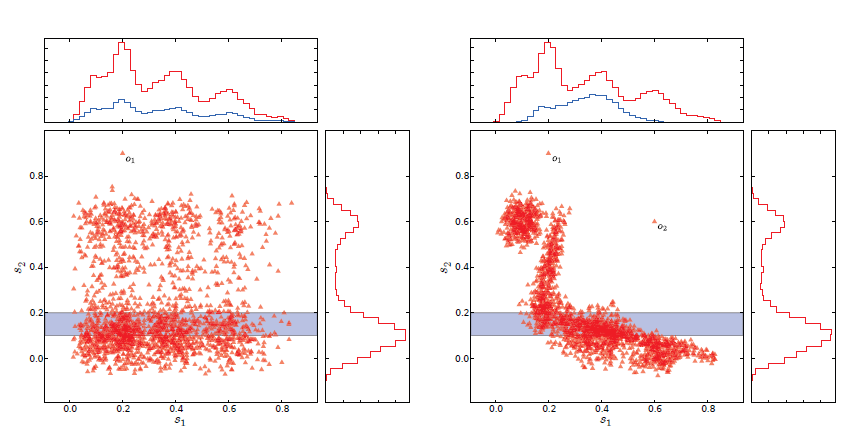
\includegraphics[scale=0.6]{imagenes/ejemplo_anomalia_probabilidad}
	\caption{Ejemplo de anomalía \cite{fabian_keller_hics:_2012}}
\end{figure}

Como se puede observar tenemos dos espacios: el izquierdo no presenta datos correlados y el derecho sí presenta correlación. Podemos ver que en ambos casos se comparte una anomalía etiquetada como $O_1$. Esta anomalía en el caso del espacio no correlado es perfectamente detectable de forma trivial observando las proyecciones de los datos en una dimensión. En cambio en el segundo caso ninguna de las dos anomalías etiquetadas $O_1 , O_2$ son detectables de esta forma trivial, pues si hacemos las proyecciones uno dimensionales ninguno de los dos datos es discordante en dichas proyecciones. Estas anomalías son las que decimos que son no triviales. En cambio si observamos los datos en una proyección de orden superior como la que estamos viendo de dimensión 2 podemos observar claramente que se salen de la correlación de datos que muestra el resto. Es aquí donde podemos ver que en el conjunto de la derecha ninguno de los puntos es una anomalía en las proyecciones de dimensión uno pero sí lo son en la proyección de dimensión 2.

Vamos por tanto a definir más formalmente este concepto especial de anomalía. Necesitamos introducir en primer lugar un poco de notación.

Partimos de un conjunto de datos $X = \{ x_1 , ... , x_n \}$ de $n$ objetos cada uno tomando $d$ valores, es decir, $x_i = (x_{s_1} , ... , x_{s_d}) \in \mathbb{R}^d$. Notamos un subespacio del conjunto de valores como:

$$S = \{ s_i | s_i \in \{ s_1 , ... , s_d \} \ con \ i\in \Delta \}$$

Dado un subespacio $S = \{ s_1 , ... , s_p \}$ notamos la proyección de los objetos del conjunto de datos como $X_{S} = \{ x_{s_1} , ... , x_{s_p} \}$.

Esta proyección está distribuida según una distribución conjunta desconocida de $S$:

$$p_{s_1 , ... , s_p} (x_{s_1} , ... , x_{s_p})$$

Notamos la distribución marginal asociada al atributo $s_i$ como:

$$p_{s_i}(x_{s_i})$$

\begin{definicion}
	Decimos que un subespacio $S$ es un espacio incorrelado si y sólo si:
	
	$$p_{s_1 , ... , s_p}(x_{s_1} , ... , x_{s_p}) = \prod_{i=1}^{p}p_{s_i}(x_{s_i})$$
\end{definicion}

Por tanto si estamos bajo la suposición de un espacio incorrelado podemos decir que la densidad esperada es:

$$p_{esp}(x_{s_1} , ... , x_{s_p}) \equiv \prod_{i=1}^{p}p_{s_i}(x_{s_i})$$

Recordemos que nuestras anomalías no triviales no están en este tipo de subespacios, si no en los correlados. Por tanto vamos a definirlo de la siguiente forma:

\begin{definicion}
	Decimos que un objeto $x_{S}$ es una anomalía no trivial respecto al subespacio $S$ si:
	
	$$p_{s_1 , ... , s_p}(x_{s_1} , ... , x_{s_p}) \ll p_{esp}(x_{s_1} , ... , x_{s_p})$$
	
	Es decir, si la probabilidad esperada es significativamente mayor que la probabilidad conjunta.
\end{definicion}

Por cómo hemos definido los espacios correlados e incorrelados es claro que no podemos tener anomalías en espacios no correlados como es evidente pues la densidad conjunta y esperada serían iguales.

Este concepto como podemos observar no comparte ninguna relación con nuestra definición de anomalías basadas en distancias por lo que es de esperar que si comparamos ambos tipos de anomalías en un conjunto de datos no obtengamos los mismos objetos.
%
%\part{Explicación de los modelos y análisis de resultados}
\label{part:explicacionmodelos_analisisrresultados}

\chapter{Modelos implementados}
\label{chapter:modelos}

En este capítulo vamos a repasar qué modelos he implementado y cómo funcionan cada uno de ellos. Primero se hará una revisión teórica de los modelos y posteriormente un análisis breve del código explicando las particularidades de las implementaciones. El contenido de esta sección se basa en los libros de Aggarwal Outlier Analysis \cite{aggarwal_outlier_2017-1} y Outlier Ensembles \cite{aggarwal_outlier_2017} y en los artículos de HICS \cite{fabian_keller_hics:_2012}, LODA \cite{pevny_loda:_2016} y OUTRES \cite{muller_statistical_2011}.

\section{Algoritmos de ensamblaje}

Los algoritmos que he implementado pertenecen a una familia concreta de algoritmos de detección de anomalías denominados como algoritmos de ensamblaje o ``Ensemble Algorithms'' en inglés. Estos algoritmos son lo equivalente a los meta-algoritmos pero destinados a la detección de anomalías. Para dar una mejor definición de qué son los algoritmos de ensamblaje vamos a introducir una clasificación de los mismos para dar las categorías que entran dentro de esta definición.

\begin{itemize}
	\item Algoritmos de ensamblaje secuenciales: En este tipo de algoritmos tenemos un algoritmos base o un conjunto de algoritmos base que se aplican de forma secuencial, de forma que las primeras ejecuciones se ven usadas o modificadas por ejecuciones futuras de algoritmos. Finalmente el resultado puede ser una combinación ponderada de las valoraciones de los algoritmos o el resultado del último de ellos.
	
	
	\begin{algorithm}[H]{\textbf{Ensamblaje secuencial:}}
		\SetAlgoLined
		
		\textbf{Entrada: } Conjunto de datos $\mathcal{D}$, Algoritmos base $\mathcal{A}_1 , ... , \mathcal{A}_r$
		
		j=1
		
		\Repeat{fin}{
			Tomamos el algoritmo $\mathcal{A}_j$ según los resultados anteriores
			
			Tomamos el conjunto de datos modificado $f_j (\mathcal{D})$ de anteriores ejecuciones
			
			Ejecutamos el algoritmo $\mathcal{A}_j$ sobre $f_j (\mathcal{D})$
			
			j=j+1
			
		}
	
		\KwResult{Combinación de los resultados}
	\end{algorithm}
	\item Algoritmos de ensamblaje independientes: En este caso se emplean o bien diferentes instancias del mismo algoritmo o bien diferentes porciones de los datos que se emplearán de forma distinta. Se puede variar la instanciación por ejemplo dependiendo del subespacio sobre el que queramos ejecutarlo o dependiendo de las características de una porción concreta de los datos.
	
	\begin{algorithm}[H]{\textbf{Ensamblaje independiente:}}
		\SetAlgoLined
		
		\textbf{Entrada: } Conjunto de datos $\mathcal{D}$, Algoritmos base $\mathcal{A}_1 , ... , \mathcal{A}_r$
		
		j=1
		
		\Repeat{fin}{
			Tomamos el algoritmo $\mathcal{A}_j$
			
			Creamos el conjunto de datos modificado $f_j (\mathcal{D})$
			
			Ejecutamos el algoritmo $\mathcal{A}_j$ sobre $f_j (\mathcal{D})$
			
			j=j+1
			
		}
		
		\KwResult{Combinación de los resultados}
	\end{algorithm}
\end{itemize}

\section{Mahalanobis Kernel}

Este algoritmo está englobado dentro de la categoría de algoritmos basados en dependencia. Esta clase de algoritmos intenta estudiar las dependencias que existen entre atributos para así poder detectar las instancias u objetos que no tienen estas dependencias y marcarlos como anomalías.

Si intentamos visualizar esta dependencia entre atributos de forma gráfica lo que observaríamos es que los datos están alineados o posicionados en hiperplanos lineales o no lineales de la siguiente forma:

\begin{figure}[H]
	\centering
	\label{hiperplano}
	\includegraphics[scale=0.8]{imagenes/hiperplano}
	\caption{Hiperplano}
\end{figure}

Esta figura es un ejemplo clásico de estudio de algoritmos como por ejemplo PCA (algoritmo que quedaría dentro de esta categoría).

\begin{figure}[H]
	\centering
	\label{hiperboloide}
	\includegraphics[scale=2.5]{imagenes/hiperboloide}
	\caption{Hiperboloide \href{https://commons.wikimedia.org/wiki/File:Circular_Hyperboloid_Of_One_Sheet_Quadric.png}{Wikimedia}}
\end{figure}

En este caso tenemos el ejemplo de un hiperboloide que no tiene una dependencia lineal, si no que presenta una dependencia de tipo cuadrático.

El método de Mahalanobis Kernel puede ser visto como una modificación de PCA. PCA básicamente dispone de dos pasos:

\begin{enumerate}
	\item Determinar un sistema ortogonal de direcciones principales y proyectar los datos sobre este sistema.
	\item Calcular la distancia entre el punto original y la proyección como su puntuación de anomalía.
\end{enumerate}

El método Mahalanobis Kernel intenta tener este mismo comportamiento en dos pasos y que ahora veremos. El algoritmo PCA es muy útil cuando los datos tienen atributos relacionados en un hiperplano, mientras que Mahalanobis Kernel funciona mejor cuando los datos están relacionados en formas más complejas como el hiperboloide que hemos enseñado. La elección de este algoritmo en vez de PCA recae en el hecho de que PCA es un algoritmo clásico y el escenario en el que mejor funciona (hiperplano) es más restrictivo que el que nos ofrece Mahalanobis Kernel con un abanico de figuras más amplio.

Vamos a describir el funcionamiento del algoritmo, pero primero vamos a introducir notación. Vamos a llamar $D$ a la matriz de datos que está centrada en la media y que tiene dimensiones $n\times d$, es decir, tenemos $n$ instancias u objetos de dimensionalidad $d$.

\begin{algorithm}[H]{\textbf{Mahalanobis Kernel}}
	\caption{Mahalanobis Kernel}
	\label{mahalanobis_kernel}
	\KwIn{$D$}
	
	$S = DD^T$.
	
	$S = Q\Delta^2 Q^T$.
	
	Almacenamos los vectores propios columna no negativos de $Q\Delta$ en una matriz $D'$
	
	Normalizamos $D'$ para que tenga media $0$ y varianza $1$.
	
	$vector\_media = media(D')$
	
	$puntuaciones = []$
	
	\ForEach{fila en D'}{
		$score = distancia(vector\_media , fila)$
		
		$puntuaciones = [puntuaciones, score]$
	}
	\KwOut{puntuaciones}
\end{algorithm}

El algoritmo comienza con la matriz de datos $D$. Se obtiene la matriz simétrica $S$ y se hace la descomposición en valores singulares. 

Con este modelo tenemos las dos fases que teníamos en PCA. Primero obtenemos una matriz $D'$ de los datos proyectados y transformados para posteriormente reportar la puntuación de anomalía como una distancia.

Veamos ahora la implementación en Python.

\begin{lstlisting}[language=Python]
def runMethod(self):
	'''
	@brief Function that executes the Kernel Mahalanobis method. The results are
	stored on the variable self.scores
	@param self
	'''
	''' Compute the S matrix of the algorithm'''
	S = np.dot(self.dataset, self.dataset.T)
	''' Now we diagonalize it'''
	Q,delta_sq,Qt = np.linalg.svd(S)
	del S
	del Qt
	''' Obtain delta as matrix'''
	delta = np.matrix(np.diag(np.sqrt(delta_sq)))
	del delta_sq
	Q = np.matrix(Q)
	''' Compute de D' matrix and normalize it'''
	Dprime = np.dot(Q,delta)
	del Q
	del delta
	Dp_std = scale(Dprime, axis=1)
	del Dprime
	''' We compute its mean on the rows to compute the deviation as the score'''
	mean = Dp_std.mean(axis=0)
	self.outlier_score=[]
	''' The score is the euclidean distance to the mean'''
	for i in range(len(Dp_std)):
		self.outlier_score.append(np.linalg.norm(mean-Dp_std[i])**2)
	self.outlier_score = np.array(self.outlier_score)
	self.calculations_done=True
\end{lstlisting}

La implementación del algoritmo se ha realizado en Python como el resto del proyecto y posteriormente se explicará en detalle cómo se ha organizado.

El algoritmo basa su implementación en la librería NumPy.

\section{TRINITY}

Este algoritmo es del segundo tipo que vimos al principio cuando hicimos una categorización de los algoritmos de ensamblaje, en concreto el algoritmo hace una combinación de tres componentes distintos. La intención de hacer esta composición de modelos es intentar obtener todos los tipos de anomalías que se puedan del conjunto y que reciban una puntuación acorde. La teoría nos dice que esta combinación de modelos nos va a proveer de un resultado más robusto que el uso de modelos aislados como discutiremos en la sección de resultados.

En concreto este algoritmo consta de tres componentes distintos:

\begin{itemize}
	\item Componente basado en distancias: este componente consta de un algoritmo que base su comportamiento en técnicas de agrupamiento o valoración por distancias como por ejemplo es el método clásico KNN. Este método lo que hace es tomar los k vecinos más cercanos y colocar como puntaje de anomalía para esa instancia como la suma de estas distancias. De esta forma los puntos que más alejados estén del resto sumarán una mayor distancia y por tanto serán más anómalos. En concreto este modelo se ha utilizado con el valor $k=5$ y con una técnica de subsampling. La técnica de subsampling consiste en no utilizar todo el conjunto de datos en el algoritmo, si no particionarlo y utilizar una pequeña muestra repitiendo este proceso y haciendo la media de las ejecuciones. De esta forma conseguimos una reducción de la varianza. Esto conlleva algunas ventajas como discutimos en la sección de sesgo y varianza anteriormente. En concreto la técnica toma 1000 particiones, ejecuta el algoritmo sobre ellas y hace la media.
	\item Componente basado en dependencia: este componente toma un algoritmo como el que hemos implementado (Mahalanobis Kernel). En este componente vamos a intentar detectar las anomalías que corresponden a datos que no siguen las relaciones entre atributos que sí tienen el resto de los objetos. Para ello he utilizado en este componente el algoritmo Mahalanobis Kernel que ya hemos explicado anteriormente incorporando la técnica de subsampling.
	\item Componente basado en densidad en subespacios: en este componente vamos a incorporar un modelo que intente buscar anomalías que lo sean en base a la densidad que tienen en alguno de los subespacios de los datos. Este hecho no nos debe ser ajeno pues es la segunda de las definiciones que hemos visto de anomalía y que hacía referencia a la función de densidad y los subespacios incorrelados y correlados. En concreto para este componente he utilizado el algoritmo IForest o Isolation Forest. Este algoritmo lo que hace es tomar de forma aleatoria un atributo y se van particionando los valores del mismo en una estructura de árbol, es decir, dividimos los datos en aquellos con un valor superior al marcado para el atributo y con un valor menor. De esta forma podemos medir cuántos pasos o lo que es lo mismo qué profundidad ha alcanzado nuestro árbol hasta llegar a dividir un objeto del resto de los datos. Este algoritmo también incorpora la técnica de subsampling.
\end{itemize}

Por último con esto hemos obtenido tres vectores o listas con la puntuación que cada componente nos ha arrojado para cada instancia. Para hacerlos comparables lo que debemos hacer es estandarizar los datos a media cero y varianza unitaria. Finalmente se realiza la media de los tres vectores de puntaje siendo esta la puntuación final devuelta por TRINITY.

Veamos la implementación de este algoritmo:

\begin{lstlisting}[language=Python]
def distanceBased(self):
	'''
	@brief Function that implements the distance based component
	@param self
	@return It returns the vector with the scores of the instances
	'''
	''' Initialize the scores'''
	scores = np.array([0]*len(self.dataset)).astype(float)
	for i in range(self.num_iter):
		knn = KNN(n_neighbors=5, contamination=self.contamination)
		''' Number in the interval [50, 1000]'''
		subsample_size = np.random.randint(50, 1001)
		sample = []
		if subsample_size>=len(self.dataset):
			sample = list(range(len(self.dataset)))
		else:
			''' Take the sample and train the model'''
			sample = np.random.choice(len(self.dataset), size=subsample_size, replace=False)
		knn.fit(self.dataset[sample])
		''' Update the score to compute the mean'''
		scores[sample]+=knn.decision_scores_
	''' Return the mean'''
	scores = scores/self.num_iter
	scores = scale(scores)
	return scores

def dependencyBased(self):
	'''
	@brief Function that implements the dependency based component
	@param self
	@return It returns the vector with the scores of the instances
	'''
	''' Initialize the scores'''
	scores = np.array([0]*len(self.dataset)).astype(float)
	for i in range(self.num_iter):
		kernel_mahalanobis = KernelMahalanobis(contamination=self.contamination)
		''' Number in the interval [50, 1000]'''
		subsample_size = np.random.randint(50, 1001)
		sample = []
		if subsample_size>=len(self.dataset):
			sample = list(range(len(self.dataset)))
		else:
			''' Take the sample and train the model'''
			sample = np.random.choice(len(self.dataset), size=subsample_size, replace=False)
		kernel_mahalanobis.fit(self.dataset[sample])
		''' Update the score to compute the mean'''
		scores[sample]+=kernel_mahalanobis.outlier_score
	''' Return the mean'''
	scores = scores/self.num_iter
	scores = scale(scores)
	return scores

def densityBased(self):
	'''
	@brief Function that implements the dependency based component
	@param self
	@return It returns the vector with the scores of the instances
	'''
	''' Initialize the scores'''
	scores = np.array([0]*len(self.dataset)).astype(float)
	for i in range(self.num_iter):
		iforest = IForest(contamination=self.contamination, behaviour="new")
		''' Number in the interval [50, 1000]'''
		subsample_size = np.random.randint(50, 1001)
		sample = []
		if subsample_size>=len(self.dataset):
			sample = list(range(len(self.dataset)))
		else:
			''' Take the sample and train the model'''
			sample = np.random.choice(len(self.dataset), size=subsample_size, replace=False)
		iforest.fit(self.dataset[sample])
		''' Update the score to compute the mean'''
		scores[sample]+=iforest.decision_scores_
	''' Return the mean'''
	scores = scores/self.num_iter
	scores = scale(scores)
	return scores

def runMethod(self):
	'''
	@brief This function is the actual implementation of TRINITY
	@param self
	'''
	''' Distance module'''
	if self.verbose:
		print("Obtaining scores with the distance module")
	distance_based = self.distanceBased()
	''' dependency module'''
	if self.verbose:
		print("Obtaining scores with the dependency module")
	dependency_based = self.dependencyBased()
	''' Density module'''
	if self.verbose:
		print("Obtaining scores with the density module")
	density_based = self.densityBased()
	
	''' Compute the mean of the three modules'''
	self.outlier_score=(distance_based + dependency_based + density_based)/3
	self.calculations_done=True
\end{lstlisting}

Todos los módulos tienen una función parecida. En primer lugar se inicializan las puntuaciones y se repite el mismo proceso de cálculo 100 veces. Se inicializa el modelo y se ajusta con una muestra de tamaño en el intervalo $[50,1000]$. Por último se hace la media de todos los cálculos y se estandarizan con la librería Sklearn.

En la función principal ``runMethod'' se ejecutan los tres módulos y se hace la media de las puntuaciones.

\section{OUTRES}

Este método entra dentro del segundo de los tipos que hemos visto en la clasificación inicial pues el objetivo es analizar los datos por subespacios. Una de las cosas que podremos ver al final cuando hagamos el estudio de los resultados es lo costoso de estos métodos, siendo este el primero que nos va a servir de ejemplo para visualizar este problema.

En primer lugar cabe decir que en el resto de algoritmos las puntuaciones reflejan el factor de anomalía en orden creciente, es decir, a mayor puntaje más anómalo es el dato y a menor puntaje menos anómalo se dice que es.

En este caso los puntajes van a estar en el intervalo $[0,1]$ siendo $0$ un puntaje para un dato lo más anómalo posible y $1$ un puntaje para un dato lo más normal posible. Daremos razones para que esto sea así cuando veamos el algoritmo.

\begin{algorithm}[H]{\textbf{OUTRES}}
	
	\KwIn{o: instancia, S: subespacio}
	
	\ForEach{$i\in (D \setminus S)$}{
	
		$S' = S\cup \{ i \}$
		
		\If{$S'$ es relevante}{
			
			$den(o, S') = \frac{1}{n} \sum_{p\in AN(o,S')} K_e (\frac{dist_{S'}(o,p)}{\epsilon (|S'|)})$
			
			$dev(o,S') = \frac{\mu - den(o,S')}{2\sigma}$
			
			\If{$dev(o,S')\geq 1$}{
				
				$r(o) = r(o) \cdot \frac{den(o,S')}{dev(o,S')}$
				
			}
		
			$OUTRES(o,S')$
			
		}
	
		\Else{
		
			Para recursividad
		
		}

	}
	
	\KwOut{r: puntajes}
	
	\caption{OUTRES}
	\label{outres}
\end{algorithm}

En primer lugar tenemos que definir qué son los espacios relevantes. Decimos que un subespacio $S$ es relevante si la proyección sobre ese subespacio no está distribuida de uniformemente. No podemos hacer un test de que toda la proyección esté distribuida uniformemente por lo que nos vamos a valer del siguiente teorema:

\begin{teorema}
	Sea $S$ un subespacio del conjunto de datos. Si $S$ está distribuido uniformemente entonces $\forall s_i \in S$ tenemos que la proyección uno-dimensional del conjunto de datos sobre $s_i$ está distribuida uniformemente.
\end{teorema}

Este teorema nos da la siguiente herramienta: si comprobamos que ninguna proyección uno-dimensional está distribuida uniformemente entonces podemos afirmar que $S$ está distribuido uniformemente. Para hacer estas comprobaciones uno-dimensionales lo hemos hecho mediante el test de Kolmogorov-Smirnov. 

Además el algoritmo incorpora un nuevo concepto. Los datos tienen mayor relevancia cuando los consideramos en subespacios y cuando los metemos dentro de lo que los autores llaman vecindarios adaptativos. La definición de un vecindario adaptativo es la siguiente:

\begin{definicion}
	Definimos para la instancia u objeto $o$ en el subespacio $S$ su vecindario adaptativo como:
	
	$$AN(o,S) = \{ p | dist_{S}(o,p)\leq \epsilon (|S|) \}$$
\end{definicion}

Donde $dist_{S}$ es la función distancia sobre los atributos $S$. Aquí tenemos una distancia máxima definida en función del cardinal del subespacio que viene dada de la siguiente forma:

$$\epsilon (|S|) = 0.5 \cdot \frac{h_{optimal}(|S|)}{h_{optimal}(2)}$$

Donde:

$$h_{optimal} (d) = (\frac{8\Gamma (\frac{d}{2} + 1)}{\pi^{\frac{d}{2}}}(d+4)(2\sqrt{\pi})^d) n^{\frac{-1}{d+4}}$$

Donde $\Gamma$ denota la función gamma y $n$ es el tamaño del conjunto de datos, es decir, el número de objetos o instancias.

Con esto ya tenemos la definición del vecindario adaptativo y el objeto de tenerlo es poder comprobar que el la instancia $o$ es relevante en el subespacio $S$ dentro de su vecindario adaptativo.

En cuanto a la definición de densidad tenemos la función $K_{\epsilon}$ que es el llamado Kernel de Epachenikov. Esta función está definida como:

$$K_{\epsilon}(x) = (1-x^2) \ \forall x<1$$

En cuanto al $\mu$ y $\sigma$ que aparecen en el cálculo de la desviación son la media y la desviación típica de las densidades en el vecindario adaptativo de $o$ en el subespacio $S$. Por tanto con la desviación estamos midiendo cómo de alejada está la instancia $o$ en densidad respecto del resto de las instancias de su vecindario adaptativo. Si esta densidad es mayor a dos desviaciones típicas entonces $dev(o,S')$ será mayor que $1$ y por tanto estaremos ante un dato anómalo.

Si este es el caso, al estar los puntajes de anomalías inicializados a 1 podemos actualizarlo multiplicando por un valor menor estricto que 1. En este caso este valor es $\frac{den(o,S')}{dev(o,S')}$. Como este valor es menor que 1 reducirá el puntaje y lo acercará más a una anomalía. De esta forma cuantas más veces se actualice su puntaje y cuanto menor puntaje obtenga con $\frac{den(o,S')}{dev(o,S')}$ más anómalo consideraremos el dato.

Finalmente si el subespacio era relevante significa que aún podemos aumentar más la dimensionalidad pues puede que nos queden subespacios de mayor orden que sigan sin estar distribuidos según una uniforme.

Como dato cabe decir que el algoritmo empieza en dimensión 2 y no en dimensión 1 pues en una única dimensión no tiene sentido estudiar la densidad ya que no vamos a sacar información de calidad.

Veamos la implementación

\begin{lstlisting}[language=Python]
def isRelevantSubspace(self, subspace, neighborhood):
	'''
	@brief Function that tells if a subspace is relevant, this is that the projection
	of the dataset over the subspace is not distributed uniformly in the neighborhood
	@param self
	@param subspace Subspace to check
	@param neighborhood neighborhood in which to check the projection
	@return It returns True if the subspace is relevant, False in other case.
	'''
	''' We check first if we have already considered this subspace. If so, it is not relevant anymore.'''
	for sub in self.checked_subspaces:
		if len(np.intersect1d(sub, subspace))==len(subspace):
			return False

	''' Make the projection'''
	projection = self.dataset[:,subspace][neighborhood]
	if len(projection)==0:
		return False
	''' We check for each subspace if the 1-dimensional data is uniformly distributed'''
	for i in range(len(subspace)):
		min = np.amin(projection[:,i].reshape(-1))
		max = np.amax(projection[:,i].reshape(-1))
		''' We do it using the Kolmogorov-Smirnov test'''
		d,p = kstest(projection[:,i], "uniform", args=(min, max-min))
		''' If the null hypothesis is not rejected, this means the data follow a uniform distribution'''
		if p<=self.alpha:
			return False
	return True

def computeHOptimal(self, d):
	'''
	@brief Function that calculates the Hoptimal
	@param self
	@param d Parameter, usually the dimensionality of the subspace
	@return It returns a numerical value.
	'''
	f1 = (8*gamma(d/2 + 1))/(np.power(np.pi, d/2))
	f2 = d+4
	f3 = np.power(2*np.sqrt(np.pi),d)
	n = len(self.dataset)
	f4 = np.power(n, -1/(d+4))
	return f1*f2*f3*f4

def computeEpsilon(self, subspace):
	'''
	@brief Function to compute the epsilon of the adapatative neighborhood
	@param self
	@params subspace Subspace considered to compute the epsilon
	@return It returns a numerical value
	'''
	return 0.5*(self.computeHOptimal(len(subspace))/self.computeHOptimal(2))

def computeNeighborhood(self, subspace, instance):
	'''
	@brief This function computes the adaptative neighborhood
	@param subspace Subspace in which to compute the neighborhood
	@param instance Instance considered as the centroid of the neighborhood (index of the element)
	@return It returns a numpy array containing the indexes of the neighborhood
	'''
	# First we compute the projection
	projection = self.dataset[:,subspace]
	# We compute a numpy array of the distances of all the elements to the instance
	tile = np.tile(projection[instance], len(self.dataset)).reshape((len(self.dataset),len(projection[instance])))
	distances = np.linalg.norm(projection-tile, axis=1)
	# We keep only the ones that are close enough (epsilon distance as max)
	neighborhood = np.where(distances<self.epsilons[len(subspace)])[0]
	# We exclude the instance itself
	return neighborhood[neighborhood!=instance]

def computeKernel(self, x):
	'''
	@brief Function that computes the Epanechnikov kernel with scalar factor 1
	@param self
	@param x Number between 0 and 1.
	@return It returns a numerical value
	'''
	return 1-np.power(x,2)

def computeDensity(self, subspace, neighborhood, instance):
	'''
	@brief This is the function that computes the density
	@param self
	@param subspace Subspace in which to compute the density
	@param neighborhood Adaptative neighborhood for the instance in the subspace
	@param instance Index of the instance considered at the moment
	@return It return a numerical value.
	'''
	# Compute the projection
	projection = self.dataset[:,subspace]
	# Compute the density
	tile = np.tile(projection[instance], len(self.dataset)).reshape((len(self.dataset),len(projection[instance])))
	return np.sum(self.computeKernel(np.linalg.norm(projection-tile, axis=1))/self.computeEpsilon(subspace))/len(self.dataset)

def computeDeviation(self, subspace, neighborhood, instance, density):
	'''
	@brief Function that computes the deviation
	@param self
	@param subspace Subspace considered to compute the deviation
	@param neighborhood Adaptative neighborhood for the instance in the subspace
	@param instance Instance to compute the deviation
	@param density Density value of the instance
	@return It returns a numerical value
	'''
	''' First we need to compute the density for all the neighbors'''
	densities = np.array([])
	for neig in neighborhood:
		local_neigborhood = self.computeNeighborhood(subspace, neig)
		densities = np.append(densities,self.computeDensity(subspace, local_neigborhood, neig))
	''' We compute the mean and the standard deviation'''
	mean = np.mean(densities)
	stdv = np.std(densities)
	''' Return the deviation'''
	return (mean-density)/(2*stdv)

def outres(self, instance, subspace):
	'''
	@brief Main loop of the outres algorithm
	@param self
	@param instance Instance to compute the outres score
	@param subspace Initial subspace of dimension 1
	'''
	''' First we compute the indexes of the features that are not used in the actual subspace'''
	available_indexes = list(set(list(range(len(self.dataset[0])))).difference(set(list(subspace))))
	''' For each available index we are going to check'''
	for index in available_indexes:
		''' We make the new subspace adding the index'''
		new_subspace = np.append(subspace, int(index)).astype(int)
		''' We compute the adaptative neighborhood'''
		neighborhood = self.computeNeighborhood(new_subspace, instance)
		''' If the subspace is relevant'''
		if self.isRelevantSubspace(new_subspace, neighborhood):
			''' Compute the density and deviation'''
			density = self.computeDensity(new_subspace, neighborhood, instance)
			deviation = self.computeDeviation(new_subspace, neighborhood, instance, density)
			''' If it is a high deviating instance in the subspace then we update the score'''
			if deviation>=1:
				if self.verbose:
					print("The instance " + str(instance+1) + " is outlying in the subspace " + str(new_subspace))
				''' The scores are equal to 1 at first and 1 means no outlierness and 0 means very outlying'''
				self.outlier_score[instance]*=density/deviation
			''' We keep the process if the subspace was relevant'''
			self.outres(instance, new_subspace)
		''' We add the subspace to the considered ones'''
		self.checked_subspaces.append(new_subspace)


def runMethod(self):
	'''
	@brief This function is the actual implementation of OUTRES
	'''
	''' First we compute all epsilons so we dont need to make this calculation more than once'''
	self.epsilons = [self.computeEpsilon(list(range(n))) for n in range(len(self.dataset[0])+1)]
	
	''' We initialize the scores to one'''
	self.outlier_score = np.ones(len(self.dataset))
	''' For each instance we run outres'''
	for i in range(len(self.dataset)):
		''' Erase checked_subspaces'''
		self.checked_subspaces = []
		if self.verbose and i%25==0:
			print("Computing the instance " + str(i+1) + "/" + str(len(self.dataset)))
		''' We run for each instance each index'''
		for j in range(len(self.dataset[0])):
			self.outres(i,np.array([j]))
	''' At the end, score 1 means no outlierness and 0 100% outlier. We make 1-score
	so we can keep the ascending order and now this will mean that 0 is no outlierness
	and 1 is very outlying.'''
	self.outlier_score = np.ones(len(self.dataset))-self.outlier_score
	self.calculations_done=True
\end{lstlisting}

\section{HICS}

HICS es otra aproximación distinta al estudio por subespacios como ha sido el algoritmo OUTRES. OUTRES intenta encontrar un subespacio interesante en el vecindario de una instancia, es decir, para cada instancia se busca el subespacio interesante para dicha instancia y no tiene por qué ser interesante para ninguna más. Esta aproximación es la opuesta pues la intención es buscar subespacios que sean interesantes en general y hacer una valoración de los datos sobre dichos subespacios.

Este algoritmo además pretende encontrar anomalías basándose en el concepto de densidad como introdujimos en la segunda definición de anomalía. Veamos primero el algoritmo en pseudocódigo para poder ir desgranándolo y explicarlo.

\begin{algorithm}[H]{\textbf{HICS}}
	
	\KwIn{D: dataset}
	
	$scores = [ \ ]$
	
	$sub = $ subespacios de alto contraste
	
	\ForEach{$S \in sub$}{
	
		Ajustamos un modelo con el algoritmo LOF con la proyección sobre $S$
		
		$scores = scores + puntaje \ LOF$
	
	}

	$scores = \frac{scores}{|sub|}$
	
	\KwOut{scores: puntajes}
	
	\caption{HICS}
	\label{hics}
\end{algorithm}

Como podemos ver el objetivo de HICS es en primer lugar obtener una serie de subespacios que sean relevantes y que hemos llamado subespacios de alto contraste. Para cada uno de estos subespacios vamos a estudiar la proyección de los datos sobre estos subespacios y vamos a obtener una puntuación de las instancias con el modelo LOF. Finalmente hacemos la media de todos estos puntajes para obtener la puntuación final. 

El modelo original está pensado para funcionar con LOF pero la teoría nos dice que podría funcionar con cualquier modelo basado en proximidad. Por tanto en la implementación desarrollada he incluido los modelos LOF, COF, CBLOF, LOCI, HBOS y SOD como alternativas entre las que elegir para la elección del modelo simple con el que obtener el puntaje.

Veamos ahora el pseudocódigo con el que obtenemos el contraste de un subespacio.

\begin{algorithm}[H]{\textbf{CalcularConstraste}}
	
	\KwIn{subespacio: subespacio, M: número de iteraciones del subsampling, $\alpha$: valor para obtener el tamaño de la muestra, $D$: conjunto de datos}
	
	$size = n \cdot \sqrt[|subespacio|]{\alpha}$
	
	$dev=0$
	
	\ForEach{$i\in [1,M]$}{
	
	$comp\_atr = aleatorio \ de \ subespacio$
	
	$sel\_obj = $ muestra aleatoria de $D$ de tamaño $size$
	
	$dev = dev + CalcularDev(comp\_atr, sel\_obj, subespacio, D)$
	
	}

	$dev = \frac{dev}{M}$
	
	\KwOut{$dev$: contraste}
	
	\caption{CalcularConstraste}
	\label{calcula_contraste}
\end{algorithm}

En resumen lo que vamos a ir haciendo es aplicar una técnica de subsampling en el algoritmo. Vamos a hacer $M$ ejecuciones para obtener el contraste tomando diferentes muestras de un tamaño fijado de antemano. Con estas muestras vamos a calcular la desviación del atributo de comparación $comp\_atr$ entre las instancias como vamos a ver ahora. Finalmente acumulamos toda esta desviación y obtenemos la media para ese subespacio. Con esto tenemos una medida de cuánto se desvían entre sí las instancias dentro de dicho subespacio.

\begin{algorithm}[H]{\textbf{CalcularDev}}
	
	\KwIn{$comp\_atr$: atributo con el que comparar, $sel\_obj$: muestra seleccionada aleatoriamente, $subespacio$: subespacio sobre el que calcular la desviación, $D$: conjunto de datos}
	
	$max = 0$
	
	\ForEach{$d\in D$}{
	
		$cum_1 = \sum_{o\in D} o[comp\_atr]$ si $o[comp\_atr]<d[comp\_atr]$
		
		$cum_2 = \sum_{o\in sel\_obj} o[comp\_atr]$ si $o[comp\_atr]<d[comp\_atr]$
		
		$f_a = \frac{cum_1}{|D|}$
		
		$f_b = \frac{cum_2}{|D|}$
		
		$subs = |f_a - f_b|$
		
		\If{$subs>max$}{
			
			$max = subs$
		
		}
	
	}
	
	\KwOut{max: máxima desviación}
	
	\caption{CalcularDev}
	\label{calcular_dev}
\end{algorithm}

Con este test lo que estamos haciendo es ver cómo se diferencia el atributo escogido para la comparación con cada instancia del resto del conjunto de datos. La idea es similar a la que expusimos cuando comentamos brevemente los Isolated Forests de ir dividiendo los datos con un valor de corte. 

Ahora ya tenemos las herramientas con las que podemos medir el contraste de un subespacio. Para ver cuáles son aquellos con mayor contraste los autores probaron dos formas quedándose finalmente con la que yo he añadido a la implementación. En primer lugar podemos pensar en algún tipo de cota que se vaya adaptando al número de subespacios o al contraste que estos vayan presentando. Esta idea finalmente fue descartada primero por no funcionar de forma satisfactoria y segundo por la dificultad de elección de la cota. La opción escogida finalmente es evaluar para cada dimensión todos los subespacios posibles, se obtiene el contraste de cada uno de ellos y se toma un número fijo de los primeros. De esta forma obtendremos por ejemplo en cada dimensión 500 candidatos. Una vez que hayamos evaluado todas las dimensiones volvemos a ordenar los subespacios por contraste (ya sin tener en cuenta la dimensionalidad) y nos quedamos con los 1000 primeros. Con esta metodología vamos a tener la certeza de que vamos a quedarnos con los 1000 subespacios con mayor contraste de entre todos los posibles. 

Veamos la implementación del algoritmo.

\begin{lstlisting}[language=Python]
def computeContrast(self, subspace):
	'''
	@brief Function that computes the contrast for a given subspace
	@param subspace Numpy array with the indexes of the features that define the subspace
	@return It returns a float representing the contrast of the subspace
	'''
	''' We set the adaptative size of the test'''
	size = int(len(self.dataset)*np.power(self.alpha, len(subspace)))
	''' Number of instances in the dataset'''
	N = len(self.dataset)
	deviation = 0
	''' We repeat the process M times'''
	for i in range(1,self.M+1):
		''' This is the comparison attribute for the test, so it will stay untouched'''
		comparison_attr=np.random.randint(low=0, high=len(subspace))
		''' List of booleans that masks the instances of the dataset selected'''
		selected_objects = np.array([True]*N)
		''' Select random indexes'''
		selected_objects[reduce(np.union1d,np.array([np.random.choice(N,size=size,replace=False) for _ in range(len(subspace)-1)]))]=False
		''' With the sample given by the mask selected_objects we compute the deviation'''
		deviation+=self.computeDeviation(subspace[comparison_attr], selected_objects, subspace)
	''' Finally the contrast is the average of all deviations'''
	return deviation/self.M

def computeDeviation(self, comparison_attr, selected_objects, subspace):
	'''
	@brief Function that computes the deviation of the marginal distribution
	given a fixed attribute, a sample and the condition given as a subspace
	@param comparison_attr This is the comparison attribute
	@param selected_objects Mask that sets a sample of the dataset
	@param subspace Subspace or condition to calculate the deviation
	@return It returns a float giving the deviation
	'''
	max = 0
	''' For each instance of the dataset'''
	for d in self.dataset:
		''' This is the cumulative value for all elements in the dataset'''
		cumul1 = np.sum(self.dataset[:,comparison_attr][self.dataset[:,comparison_attr]<d[comparison_attr]])
		''' This is the cumulative value for the selected_objects aka the sample'''
		sel = self.dataset[:,comparison_attr][selected_objects]
		cumul2 = np.sum(sel[sel<d[comparison_attr]])
		''' Finally we compute the average in both cases'''
		fa = cumul1/len(self.dataset)
		fb = cumul2/len(self.dataset)
		''' The difference in absolute value is the deviation'''
		subs = np.absolute(fa-fb)
		''' We return the biggest of the deviations obtained'''
		if subs>max:
			max = subs
	return max

def hicsFramework(self):
	'''
	@brief This function computes the high contrast subspaces on which to score the outlier
	@return It returns a numpy array containing the high contrast subspaces
	'''
	''' Ordered subspaces by dimension type: list of numpy arrays of numpy arrays
	 this means that in each positions there would be the subspaces of the corresponding
	 dimension in the form of a list of subspaces which are numpy arrays'''
	all_subspaces = []
	''' Record of the contrast for each subspace in each dimension, same shape as all_subspaces'''
	all_contrasts = []
	''' For all dimensions starting from dimension 2 (correlation has no sense on dimension 1)'''
	for dimension in range(2,len(self.dataset[0])):
		if self.verbose:
			print("Computing subspaces in dimension " + str(dimension) + "/" + str(len(self.dataset[0])))
		candidates = []
		contrasts = []
		''' This list will keep the indexes of the redundant subspaces, those are d-dimensional subspaces with d+1-dimensional
		 subspaces containing them with higher contrast'''
		redundant = []
		''' For dimension 2 we just obtain all possible indexes and make all combinations'''
		if dimension==2:
			''' Calculate the candidates as all possible combinations'''
			indexes = list(range(len(self.dataset[0])))
			candidates = np.array([np.array(list(comb)) for comb in list(combinations(indexes,dimension))])
			''' Compute the contrasts'''
			cont = 0
			p = Pool(self.numThreads)
			while cont+self.numThreads<len(candidates):
				contrasts = contrasts + p.map(self.computeContrast,candidates[cont:cont+self.numThreads])
				cont+=self.numThreads
				print("Computed " + str(cont) + "/" + str(len(candidates)))
			p = Pool(len(candidates)-cont)
			contrasts = contrasts + p.map(self.computeContrast,candidates[cont:])
			print("Computed " + str(len(candidates)) + "/" + str(len(candidates)))
		else:
			''' We need to calculate now the indexes starting from a previous subspace
			 We record the parent of each subspace to check for redundancy'''
			parents = []
			''' For all subspaces with one dimension less'''
			for i in range(len(all_subspaces[-1])):
				''' We only consider new indexes, those are the ones not uses in the father subspace'''
				indexes = list(set(list(range(len(self.dataset[0])))).difference(set(all_subspaces[-1][i])))
				''' For each new index'''
				for ind in indexes:
				''' We calculate the new candidate as the same subspace appending the index'''
				new_can = np.append(all_subspaces[-1][i],ind)
				''' Now we check that the candidate wasn't in the list before'''
				new = True
				for previous in candidates:
					if len(np.intersect1d(previous,new_can))==len(new_can):
						new = False
				if new:
					candidates.append(new_can)
					parents.append(i)
			''' Compute the contrasts'''
			cont = 0
			p = Pool(self.numThreads)
			while cont+self.numThreads<len(candidates):
				contrasts = contrasts + p.map(self.computeContrast,candidates[cont:cont+self.numThreads])
				cont+=self.numThreads
				print("Computed " + str(cont) + "/" + str(len(candidates)))
			p = Pool(len(candidates)-cont)
			contrasts = contrasts + p.map(self.computeContrast,candidates[cont:])
			print("Computed " + str(len(candidates)) + "/" + str(len(candidates)))
			
			''' Check for redundancy'''
			for i in range(len(parents)):
				if contrasts[i]>all_contrasts[-1][parents[i]]:
					redundant.append(parents[i])
		
		candidates = np.array(candidates)
		contrasts = np.array(contrasts)
		''' If there are redundant subspaces'''
		if redundant!=[]:
			if self.verbose:
				print("Now deleting redundant subspaces in dimension " + str(dimension) + ", " + str(len(redundant)) + " subspaces removed.")
		''' Delete those ones'''
		non_redundant_sub = np.delete(all_subspaces[-1], redundant)
		''' Update the subspaces'''
		all_subspaces[-1]=non_redundant_sub
		''' Sort from higher contrast to lower and only get numCandidates number of subspaces if available'''
		if len(candidates)>self.numCandidates:
			all_subspaces.append(candidates[contrasts.argsort()[-self.numCandidates:][::-1]])
			all_contrasts.append(contrasts[contrasts.argsort()[-self.numCandidates:][::-1]])
		else:
			all_subspaces.append(candidates)
			all_contrasts.append(contrasts)
	''' We flatten the numpy array to obtain only a list of subspaces and contrasts'''
	subspaces = np.array(all_subspaces).flatten()
	contrasts = np.array(all_contrasts).flatten()
	''' We only give the maxOutputSpaces with higher contrast if available'''
	if len(subspaces)>self.maxOutputSpaces:
		return subspaces[contrasts.argsort()[-self.maxOutputSpaces:][::-1]]
	return subspaces

def runMethod(self):
	'''
	@brief This function is the actual implementation of HICS
	'''
	if self.verbose:
		print("Calculating the subspaces\n")
	''' First we obtain the high contrast subspaces'''
	subspaces = self.hicsFramework()
	
	if self.verbose:
		print("Now calculating the scoring\n")
	''' We initialize the scores for each instance as 0'''
	scores = np.zeros(len(self.dataset))
	''' For each subspace'''
	for sub in subspaces:
		''' We place the corresponding scorer according to parameter'''
		scorer = None
		if self.outlier_rank=="lof":
			scorer = LOF()
		elif self.outlier_rank=="cof":
			scorer = COF()
		elif self.outlier_rank=="cblof":
			scorer = CBLOF()
		elif self.outlier_rank=="loci":
			scorer = LOCI()
		elif self.outlier_rank=="hbos":
			scorer = HBOS()
		elif self.outlier_rank=="sod":
			scorer = SOD()
		''' Fits the scorer with the dataset'''
		scorer.fit(self.dataset[:,sub])
		''' Adds the scores obtained to the global ones'''
		scores = scores+scorer.decision_scores_
	''' Compute the average'''
	self.outlier_score = scores/len(subspaces)
	''' Marks the calculations as done'''
	self.calculations_done=True
\end{lstlisting}

\section{LODA}

LODA es un algoritmo que entra en la categoría de los algoritmos que involucran histogramas. Aún no hemos visto ningún algoritmo de este tipo, por lo que no hemos discutido el funcionamiento de estos algoritmos. Cuando hacemos un histograma de los datos estudiamos la distribución de probabilidad de los datos y por tanto podemos ver si éstos están en las colas en algún atributo o proyección o si están en el centro de la distribución. Con esto podemos saber si el dato es o no anómalo. En concreto LODA emplea una serie de proyecciones uno-dimensionales sobre las que se estudia la distribución. 

En primer lugar vamos a ver cómo se obtienen los vectores que nos dan las proyecciones uno-dimensionales.

\begin{algorithm}[H]{\textbf{ProyeccionesAleatorias}}
	
	\KwIn{$d$: dimension, $D$: dataset, $k$: número de histogramas y proyecciones}
	
	$no\_neg = [\sqrt{d}]$
	
	$proyecciones = [ \ ]$
	
	\ForEach{$i\in [1,k]$}{
	
		$ind = $ $no\_neg$ indices aleatorios en $[0,d]$
		
		$proy = $ vector con ceros en todas las posiciones menos en ind, donde hay valores sacados de una normal $\mathcal{N}(0,1)$
		
		$proyecciones = [proecciones, proy]$

	}
	
	\KwOut{$proyecciones$: proyecciones}
	
	\caption{ProyeccionesAleatorias}
	\label{proyecciones_aleatorias}
\end{algorithm}

En LODA tenemos un parámetro $k$ que nos indica el número de proyecciones e histogramas que vamos a desarrollar. Esto nos va a dar más o menos muestras como haríamos con una técnica de subsampling tradicional. 

Una vez que tenemos estos vectores de proyección vamos a ver cómo generamos los histogramas a partir de ellos.

\begin{algorithm}[H]{\textbf{ObtenerHistogramas}}
	
	\KwIn{$D$: dataset, $\{w_i\}_{i=1}^{k}$: vectores de proyecciones, $k$: numero de histogramas y vectores de proyección}
	
	Inicializamos los histogramas $\{h_i\}_{i=1}^{k}$
	
	\For{$j=1 \rightarrow |D|$}{
	
		\For{$i=1\rightarrow k$}{
		
			$z_i = x_j^T w_i$	
			
			Actualiza el histograma $h_i$ con $z_i$

		}

	}
	
	\KwOut{$\{h_i\}_{i=1}^{k}$: histogramas}
	
	\caption{ObtenerHistogramas}
	\label{obtener_histogramas}
\end{algorithm}

Con esto ya tenemos tanto las proyecciones como los histogramas, por lo que sólo queda ver cómo obtenemos las puntuaciones de anomalías de los datos.

\begin{algorithm}[H]{\textbf{LODA}}
	
	\KwIn{$x$: instancia, $\{h_i\}_{i=1}^{k}$: histogramas, $\{w_i\}_{i=1}^{k}$: vectores de proyección}
	
	\For{$i=1\rightarrow k$}{
	
		$z_i = x^T w_i$
		
		Obtenemos $p_i = p_i (z_i)$ del histograma $h_i$

	}

	$f = \frac{-1}{k} \sum_{i=1}^{k}\log (p_i (z_i))$
	
	\KwOut{$f$: puntaje de anomalía de $x$}
	
	\caption{LODA}
	\label{loda}
\end{algorithm}

Finalmente ya tenemos el algoritmo LODA completo. Cuando estamos evaluando una instancia obtenemos la probabilidad de que su proyección uno-dimensional ocurra. Con esta probabilidad si hacemos el logaritmo cuanto más cerca esté de $0$ más cerca estará el valor de $-\infty$ y por tanto mayor va a ser nuestro puntaje anómalo de dicha instancia.

Ahora que ya tenemos el algoritmo completo vamos a ver la implementación:

\begin{lstlisting}[language=Python]
def getRandomProjections(self, dimension):
	'''
	@brief Function that computes and returns the random projections
	@param self
	@param dimension Dimensionality of the dataset (int)
	@return It returns a list with numpy arrays as projections
	'''
	''' Number of non-negative elements in the projection'''
	non_neg = int(np.ceil(np.sqrt(dimension)))
	projections = []
	''' We are going to compute k projections'''
	for i in range(self.k):
		''' Select non_neg random indexes to make the projection'''
		ind = np.random.choice(dimension, replace=False, size=non_neg)
		''' Initialize it to zeroes'''
		proj = np.zeros(dimension)
		''' The non-negative elements are drawn from a normal distribution'''
		proj[ind]=np.random.normal(size=non_neg)
		projections.append(proj)
	return projections

def getBin(self, hist_limits, value):
	'''
	@brief Function that given a value, it returns the bin it belongs to for the histogram
	@param self
	@param hist_limits Limits for each bin of the histogram
	@param value Value to check for the bin
	@return It returns the index corresponding to the bin
	'''
	bin=-1
	for i in range(len(hist_limits)):
		if value<hist_limits[i]:
			bin=i
			break
	return bin-1

def runMethod(self):
	'''
	@brief This is the implementation of the LODA algorithm
	'''
	''' We compute first all projections'''
	random_projections = self.getRandomProjections(len(self.dataset[0]))
	''' Initialize the histograms and the projected data'''
	histograms = [[]]*self.k
	Z = [[]]*self.k
	''' For each instance of the dataset'''
	for j in range(len(self.dataset)):
		''' For each projection'''
		for i in range(self.k):
			''' Compute the 1D projection'''
			Z[i].append(np.dot(self.dataset[j].T, random_projections[i]))
	''' Compute the k histograms with the data'''
	for i in range(self.k):
		histograms[i]=np.histogram(Z[i], bins = self.n_bins)
	
	''' Initialize the scores to zero'''
	self.outlier_score = np.array([0]*len(self.dataset)).astype(float)
	''' For each instance'''
	for i in range(len(self.dataset)):
		prob = []
		''' For each histogram'''
		for j in range(self.k):
			''' Compute the projection'''
			z = np.dot(self.dataset[i].T, random_projections[j])
			''' Check the bin for the projection'''
			bin = self.getBin(histograms[j][1], z)
			''' Obtain the probability linked to z in the histogram'''
			prob.append(histograms[j][0][bin]/np.sum(histograms[j][0]))
		prob = np.array(prob)
		''' Compute the score with the probabilities'''
		if 0. in prob:
			self.outlier_score[i] = float("inf")
		else:
			self.outlier_score[i] = -np.sum(np.log(prob))/self.k
	self.calculations_done=True
\end{lstlisting}

\section{Implementación}

Todos los algoritmos están implementados utilizando una clase base llamada EnsembleTemplate:

\begin{lstlisting}[language=Python]
class EnsembleTemplate:
'''
Template class for the ensemble anomaly detectors.
'''

def __init__(self, contamination=0.1):
	'''
	Init template
	'''
	pass

def fit(self, dataset):
	'''
	Function to set the dataset and execute the algorithm
	'''
	self.dataset = dataset
	self.outlier_score = [0]*len(self.dataset)
	self.outliers = []
	self.runMethod()
	return self

def runMethod(self):
	'''
	Function to run the method implemented
	'''
	pass

def getRawScores(self):
	'''
	Function that gets the raw scores
	'''
	return self.outlier_score

def getOutliersBN(self, noutliers):
	'''
	Function that gets the noutliers instances of the most outlying data
	'''
	return self.outliers

def getOutliers(self):
	pass
\end{lstlisting}

El esqueleto de todas las clases que implementan los algoritmos de los que hemos hablado es este. En primer lugar todas las clases tienen un constructor en el que se pasan los parámetros de los modelos en caso de haberlos. En segundo lugar tenemos una función fit. El cometido de esta función es inicializar las puntuaciones, pasar el dataset al objeto de la clase para que se guarde y por último ejecutar el método que implementa.

La función principal es la función runMethod que es la que implementa la ejecución del algoritmo en sí. Esta función no está pensada para ser llamada externamente si no desde fit. 

Por último tenemos tres funciones más. La primera de ellas nos da el vector que contiene los puntajes de las anomalías. La segunda función nos da los ``noutliers'' elementos con mayor puntaje y la tercera nos devuelve las instancias anómalas basándose en un parámetro que llamamos contaminación. 

El parámetro de contaminación no es más que una estimación del porcentaje de anomalías que pensamos que va a tener el conjunto de datos. Por tanto si el parámetro de contaminación fuera por ejemplo $0.1$ entonces esta función devolvería el primer $10\%$ con mayor valor de puntaje de anomalía.

Toda la implementación del trabajo se encuentra alojada en GitHub en \href{https://github.com/nacheteam/Ensemble-Outlier-Analysis}{\textbf{\underline{este repositorio}}}.
%
%\chapter{Experimentación y Resultados}
\label{chapter:experimentacion_resultados}

\section{Conjuntos de datos}

Para comenzar la experimentación vamos a hacer un repaso de los conjuntos de datos y la técnica seguida para realizar la misma. En primer lugar cabe decir que al ser un problema no supervisado en origen no tendríamos forma de saber nuestro acierto en el problema. En este tipo de casos hay dos aproximaciones: estimar el acierto o utilizar conjuntos que sí están clasificados y obtener de esta forma el acierto. La segunda de las alternativas es la que vamos a seguir en este estudio y es la que se suele denominar como problema semi-supervisado. 

Para tomar este camino necesitamos conjuntos en los que tengamos disponible la clasificación de datos anómalos y no anómalos. Estos conjuntos de datos han sido tomados de la web Outlier Detection Datasets \cite{shebuti_ryana_odds_2016}, librería mantenida por la universidad Stony Brooks.

Estos conjuntos de datos están en formato Matlab, formato que puede ser fácilmente leído por la librería SciPy. Estos conjuntos de datos vienen con información de cabecera, versión e incluso algunos con una breve descripción o resumen si dispusieran de ella. Lo importante es que los datos vienen divididos en dos, primero un vector que contiene una lista con los vectores que componen los datos y en segundo lugar un vector con las etiquetas donde $0$ significa que el dato no es anómalo y $1$ que sí lo es.

\begin{figure}[H]
	\centering
	\includegraphics[scale=0.8]{imagenes/datasets_matlab}
	\caption{Contenido de los conjuntos de datos}
	\label{dataset_matlab}
\end{figure}

Como podemos ver ``X'' contiene el conjunto de datos y el campo ``y'' contiene las etiquetas para los mismos.

En algunos de estos conjuntos de datos podemos encontrar lo que conocemos como valores perdidos o en inglés ``missing values''. Estos valores vienen reflejados con ``NAN'' en los conjuntos. Estos valores no sólo no nos son de interés si no que además nuestros modelos no están preparados para poder trabajar con ellos por lo que tenemos que decidir que transformación aplicamos para poder emplear los conjuntos de datos. La decisión tomada para estos valores ha sido la de eliminar las instancias que presenten valores perdidos. Esta decisión se basa en que, si estas instancias son anómalas no tenemos forma alguna de tratar con ellas porque no disponen de valores numéricos en sus campos y por tanto nuestros modelos no son aptos para resolver el conflicto. Esto no excluye el hecho de que estas instancias puedan ser anomalías reales. Por ejemplo pensemos en un sistema de frenos que sufre una rotura de alguno de sus sistemas. Si estos sistemas poseen sensores que recopilan datos es muy probable que estos sensores no tomen valores y por tanto dispongamos de valores perdidos precisamente porque la instancia es anómala. Esto se discutirá un poco más en profundidad cuando hablemos del trabajo futuro, de momento la decisión ha sido suprimir estas instancias.

Dentro de todos los conjuntos de datos que contiene la librería nosotros vamos a utilizar los siguientes:

\begin{table}[H]
	\centering
	\begin{tabular}{|l|l|l|}
		\hline
		\multicolumn{1}{|c|}{{\ul \textbf{Nombre}}} & \multicolumn{1}{c|}{{\ul \textbf{Dimensionalidad}}} & \multicolumn{1}{c|}{{\ul \textbf{Número de instancias}}} \\ \hline
		annthyroid                                  & 6                                                   & 7200                                                     \\ \hline
		arrhythmia                                  & 274                                                 & 452                                                      \\ \hline
		breastw                                     & 9                                                   & 683                                                      \\ \hline
		cardio                                      & 21                                                  & 1831                                                     \\ \hline
		glass                                       & 9                                                   & 214                                                      \\ \hline
		ionosphere                                  & 33                                                  & 351                                                      \\ \hline
		letter                                      & 32                                                  & 1600                                                     \\ \hline
		lympho                                      & 18                                                  & 148                                                      \\ \hline
		mammography                                 & 6                                                   & 11183                                                    \\ \hline
		mnist                                       & 100                                                 & 7603                                                     \\ \hline
		musk                                        & 166                                                 & 3062                                                     \\ \hline
		optdigits                                   & 64                                                  & 5216                                                     \\ \hline
		pendigits                                   & 16                                                  & 6870                                                     \\ \hline
		pima                                        & 8                                                   & 768                                                      \\ \hline
		satellite                                   & 36                                                  & 6435                                                     \\ \hline
		satimage-2                                  & 36                                                  & 5803                                                     \\ \hline
		speech                                      & 400                                                 & 3686                                                     \\ \hline
		thyroid                                     & 6                                                   & 3772                                                     \\ \hline
		vertebral                                   & 6                                                   & 240                                                      \\ \hline
		vowels                                      & 12                                                  & 1456                                                     \\ \hline
		wbc                                         & 30                                                  & 378                                                      \\ \hline
		wine                                        & 13                                                  & 129                                                      \\ \hline
	\end{tabular}
	\caption{Tabla con información de los conjuntos de datos}
\end{table}

Como podemos ver hay algunos conjuntos con un tamaño razonablemente grande tanto en dimensionalidad como en número de instancias. Esto será discutido modelo por modelo pues los algoritmos basados en subespacios tienen una complejidad dependiente del factorial de la dimensionalidad, es decir, a partir de una cierta dimensionalidad el tiempo que consumen estos algoritmos es demasiado alto.

\section{Experimentación}

Sobre estos conjuntos de datos hemos ejecutado nuestros cinco modelos implementados: HICS, OUTRES, Mahalanobis Kernel, Trinity y LODA. Sobre estas ejecuciones se ha recopilado el porcentaje de acierto sobre ellos, el tiempo consumido en la ejecución y las propias puntuaciones dadas sobre estos conjuntos de datos por los modelos.

Para poder hacer la comparativa con los datos de nuestros modelos he tomado modelos clásicos. Estos modelos se han cogido de la librería PyOD \cite{zhao_pyod:_2019}. De esta librería se han tomado 10 modelos: Angle-Based Outlier Detection (ABOD), Connectivity-Based Outlier Factor (COF), Histogram-Based Outlier Score (HBOS), K Nearest Neighbors (KNN), Local Outlier Factor (LOF), Minimum Covariance Determinant (MCD), One-Class Support Vector Machines (OCSVM), Principal Component Analysis (PCA), Subspace Outlier Detection (SOD) y Stochastic Outlier Selection (SOS). Sobre estos modelos se ha recopilado exactamente la misma información que sobre los nuestros, es decir, el acierto, el tiempo consumido y las puntuaciones de las instancias.

En cuanto a OUTRES podemos estudiar cuándo un subespacio es importante para una instancia completa. Por tanto hemos lanzado otro experimento para intentar analizar los subespacios que son más relevantes para una determinada instancia.

\section{Resultados}

En primer lugar vamos a ver los resultados que obtenemos de todos los modelos sobre todos los conjuntos de datos. Se muestra un gráfico de barras por cada conjunto de datos con el desempeño de cada modelo. Cabe decir que tanto OUTRES como HICS son algoritmos como hemos comentado con una eficiencia muy mala en tiempo. Al ser su complejidad en tiempo dependiente del factorial de la dimensionalidad sólo hemos ejecutado el algoritmo en conjuntos de datos de baja dimensionalidad para poder completar dicha ejecución en un tiempo razonable, aunque como veremos hay algunos conjuntos de datos cuya ejecución ha llevado varias horas.

Veamos primero todos los gráficos con los resultados para poder analizarlos y particularizar posteriormente.

\begin{figure}[H]
	\centering
	\includegraphics[scale=0.7]{imagenes/imgs-exp1/accuracy/annthyroid}
	\caption{Porcentaje de acierto sobre el conjunto de datos annthyroid}
	\label{annthyroid_accuracy}
\end{figure}

\begin{figure}[H]
	\centering
	\includegraphics[scale=0.7]{imagenes/imgs-exp1/accuracy/arrhythmia}
	\caption{Porcentaje de acierto sobre el conjunto de datos arrhythmia}
	\label{arrhythmia_accuracy}
\end{figure}

\begin{figure}[H]
	\centering
	\includegraphics[scale=0.7]{imagenes/imgs-exp1/accuracy/breastw}
	\caption{Porcentaje de acierto sobre el conjunto de datos breastw}
	\label{breastw_accuracy}
\end{figure}

\begin{figure}[H]
	\centering
	\includegraphics[scale=0.7]{imagenes/imgs-exp1/accuracy/cardio}
	\caption{Porcentaje de acierto sobre el conjunto de datos cardio}
	\label{cardio_accuracy}
\end{figure}

\begin{figure}[H]
	\centering
	\includegraphics[scale=0.7]{imagenes/imgs-exp1/accuracy/glass}
	\caption{Porcentaje de acierto sobre el conjunto de datos glass}
	\label{glass_accuracy}
\end{figure}

\begin{figure}[H]
	\centering
	\includegraphics[scale=0.7]{imagenes/imgs-exp1/accuracy/ionosphere}
	\caption{Porcentaje de acierto sobre el conjunto de datos ionosphere}
	\label{ionosphere_accuracy}
\end{figure}

\begin{figure}[H]
	\centering
	\includegraphics[scale=0.7]{imagenes/imgs-exp1/accuracy/letter}
	\caption{Porcentaje de acierto sobre el conjunto de datos letter}
	\label{letter_accuracy}
\end{figure}

\begin{figure}[H]
	\centering
	\includegraphics[scale=0.7]{imagenes/imgs-exp1/accuracy/lympho}
	\caption{Porcentaje de acierto sobre el conjunto de datos lympho}
	\label{lympho_accuracy}
\end{figure}

\begin{figure}[H]
	\centering
	\includegraphics[scale=0.7]{imagenes/imgs-exp1/accuracy/mammography}
	\caption{Porcentaje de acierto sobre el conjunto de datos mammography}
	\label{mammography_accuracy}
\end{figure}

\begin{figure}[H]
	\centering
	\includegraphics[scale=0.7]{imagenes/imgs-exp1/accuracy/mnist}
	\caption{Porcentaje de acierto sobre el conjunto de datos mnist}
	\label{mnist_accuracy}
\end{figure}

\begin{figure}[H]
	\centering
	\includegraphics[scale=0.7]{imagenes/imgs-exp1/accuracy/musk}
	\caption{Porcentaje de acierto sobre el conjunto de datos musk}
	\label{musk_accuracy}
\end{figure}

\begin{figure}[H]
	\centering
	\includegraphics[scale=0.7]{imagenes/imgs-exp1/accuracy/optdigits}
	\caption{Porcentaje de acierto sobre el conjunto de datos optdigits}
	\label{optdigits_accuracy}
\end{figure}

\begin{figure}[H]
	\centering
	\includegraphics[scale=0.7]{imagenes/imgs-exp1/accuracy/pendigits}
	\caption{Porcentaje de acierto sobre el conjunto de datos pendigits}
	\label{pendigits_accuracy}
\end{figure}

\begin{figure}[H]
	\centering
	\includegraphics[scale=0.7]{imagenes/imgs-exp1/accuracy/pima}
	\caption{Porcentaje de acierto sobre el conjunto de datos pima}
	\label{pima_accuracy}
\end{figure}

\begin{figure}[H]
	\centering
	\includegraphics[scale=0.7]{imagenes/imgs-exp1/accuracy/satellite}
	\caption{Porcentaje de acierto sobre el conjunto de datos satellite}
	\label{satellite_accuracy}
\end{figure}

\begin{figure}[H]
	\centering
	\includegraphics[scale=0.7]{imagenes/imgs-exp1/accuracy/satimage-2}
	\caption{Porcentaje de acierto sobre el conjunto de datos satimage-2}
	\label{satimage-2_accuracy}
\end{figure}

\begin{figure}[H]
	\centering
	\includegraphics[scale=0.7]{imagenes/imgs-exp1/accuracy/speech}
	\caption{Porcentaje de acierto sobre el conjunto de datos speech}
	\label{speech_accuracy}
\end{figure}

\begin{figure}[H]
	\centering
	\includegraphics[scale=0.7]{imagenes/imgs-exp1/accuracy/thyroid}
	\caption{Porcentaje de acierto sobre el conjunto de datos thyroid}
	\label{thyroid_accuracy}
\end{figure}

\begin{figure}[H]
	\centering
	\includegraphics[scale=0.7]{imagenes/imgs-exp1/accuracy/vertebral}
	\caption{Porcentaje de acierto sobre el conjunto de datos vertebral}
	\label{vertebral_accuracy}
\end{figure}

\begin{figure}[H]
	\centering
	\includegraphics[scale=0.7]{imagenes/imgs-exp1/accuracy/vowels}
	\caption{Porcentaje de acierto sobre el conjunto de datos vowels}
	\label{vowels_accuracy}
\end{figure}

\begin{figure}[H]
	\centering
	\includegraphics[scale=0.7]{imagenes/imgs-exp1/accuracy/wbc}
	\caption{Porcentaje de acierto sobre el conjunto de datos wbc}
	\label{wbc_accuracy}
\end{figure}

\begin{figure}[H]
	\centering
	\includegraphics[scale=0.7]{imagenes/imgs-exp1/accuracy/wine}
	\caption{Porcentaje de acierto sobre el conjunto de datos wine}
	\label{wine_accuracy}
\end{figure}

Como podemos observar los resultados que hemos obtenido han sido variados. En primer lugar cabe justificar algunos valores en función de la dificultad de la tarea. Como hemos comentado en la parte teórica el concepto de anomalía es algo difícil de enmarcar por lo que también es algo complejo de detectar y por tanto en función de cada conjunto de datos puede que detectemos mejor o peor sus anomalías. Por eso por ejemplo tenemos conjuntos de datos como \ref{glass_accuracy} en los que el mejor de los resultados apenas es poco más de un 20\% o \ref{optdigits_accuracy} en el que ni siquiera llegamos a dicho 20\%. Esto no es más que el reflejo de la dificultad del problema. Lo interesante de este estudio es si conseguimos mejorar en algún caso con respecto a los modelos tradicionales y la respuesta es que alguno de los modelos que hemos implementado superan en ciertos conjuntos de datos a los clásicos.

Hemos conseguido con nuestros modelos conseguir la mejor puntuación en $8$ de $22$ conjuntos de datos. Este resultado puede no parecer significativo pero debemos considerar que tenemos el doble de modelos clásicos que de modelos de ensamblaje y que ni mucho menos todos los algoritmos clásicos están al mismo nivel. Además tenemos algoritmos clásicos de todos los tipos por lo que como podemos ver en algunos conjuntos de datos no funcionan todos bien pero alguno destaca y viceversa. 

Como podemos ver en los $22$ conjuntos de datos que hemos probado los dos modelos que peores resultados nos han arrojado de los 5 implementados son HICS y OUTRES, es decir, los dos modelos basados en subespacios que hemos implementado. Esto no quiere decir que los dos modelos sean de poca relevancia. La idea del estudio por subespacio es algo razonable y que puede arrojar buenos resultados, pero quizás no hemos utilizado para estos dos algoritmos ningún conjunto de datos conveniente. Además, los algoritmos de subespacios presentados son un poco rígidos en esta concepción sin querer salirse de la misma. Por ejemplo HICS obtiene sobre todo según hemos  visto anomalías que no son triviales o claramente basadas en la definición de distancias. Es por esto que, aunque lo hayamos probado como un modelo sólo, pienso que es un algoritmo más idóneo para aplicarlo en conjunción con otro tipo de algoritmos. Por ejemplo sería interesante aplicar un algoritmo basado en subespacios después de aplicar Mahalanobis Kernel puesto que este modelo y Trinity son los más fiables de los 5 que hemos estudiado. Por ejemplo podemos ver que en \ref{arrhythmia_accuracy}, \ref{breastw_accuracy}, \ref{mnist_accuracy} o \ref{satimage-2_accuracy} tanto Trinity como Mahalanobis Kernel funcionan muy bien. 

Hay un dato bastante interesante en la comparativa entre Mahalanobis Kernel y Trinity. Como hemos visto en la explicación de los modelos Trinity tiene a Mahalanobis Kernel en el primer componente. Esto en los resultados se refleja en que Trinity en general obtiene mejores resultados que Mahalanobis Kernel. El segundo componente vimos que era KNN, comparando con este modelo vemos que los resultados que obtiene Trinity son al menos iguales aunque en varios conjuntos son mejores los de Trinity que los de KNN. Por último el tercer componente de Trinity es IForest que no ha entrado dentro de esta comparativa por ser un modelo de ensamblaje también y por tanto carece de sentido contraponerlo con nuestros modelos. Esto nos está mostrando que efectivamente la combinación de modelos hace que los resultados sean más robustos obteniendo mejores resultados en general o en el peor caso manteniendo aproximadamente los resultados del modelo individual.

Por último podemos ver que LODA en general no tiene unos resultados muy espectaculares. Aún así consigue ponerse en cabeza en \ref{breastw_accuracy}, \ref{cardio_accuracy}, \ref{mammography_accuracy}, \ref{pima_accuracy} y \ref{wbc_accuracy}. En el resto de conjuntos de datos no obtiene unos buenos resultados, lo que nos está diciendo que funciona muy bien en conjuntos de datos adecuados.

Vamos a ver ambos conjuntos de datos para comprobar la razón de este comportamiento.

\begin{figure}[H]
	\centering
	\includegraphics[scale=0.7]{imagenes/breastw}
	\caption{Proyección de breastw}
	\label{breastw}
\end{figure}

\begin{figure}[H]
	\centering
	\includegraphics[scale=0.7]{imagenes/glass}
	\caption{Proyección de glass}
	\label{glass}
\end{figure}

Como podemos ver en las figuras primeras LODA funciona muy bien sobre el conjunto de datos breastw y muy mal sobre el conjunto de datos glass. Para comprobar la forma de estos dos conjuntos de datos hemos dibujado la proyección en dos dimensiones utilizando la técnica TSNE. Como podemos observar en el conjunto de datos breastw tenemos las anomalías muy separadas del resto de los datos (siendo las anomalías los datos en rojo) mientras que en glass están dentro de los datos que consideraríamos normales. Esto nos está diciendo que cuanto mayor sea la aparición de anomalías del tipo basadas en distancias mejor es el desempeño de LODA. 

Como podemos ver casi todos los modelos fallan en conjuntos de datos como optdigits. Veamos su proyección para intentar entenderlo.

\begin{figure}[H]
	\centering
	\includegraphics[scale=0.7]{imagenes/optdigits}
	\caption{Proyección de optdigits}
	\label{optdigits}
\end{figure}

Podría parecer que el mal desempeño de los algoritmos sea completamente ilógico al ver que las anomalías están completamente diferenciadas de los datos. Como podemos ver no sólo están separadas del resto de los datos, si no que además están muy apiñadas entre sí. Esto es un inconveniente tremendo en la detección de anomalías. Como vimos en la primera de las definiciones las anomalías deben ser datos cuya distancia al centroide sea alta cosa que no pasa en este conjuntos de datos. Si nos fijamos en la segunda definición estamos intentando estudiar la densidad de datos para ver la anomalía pero este clúster tiene una alta densidad con lo que los datos no entrarían en la definición. Este conjunto de datos refleja perfectamente la complejidad del problema. Tenemos empíricamente determinadas las anomalías pero no entran claramente en las definiciones que podemos proveer de las mismas con lo que nos es difícil clasificarlas.

HICS tiene un desempeño razonablemente bueno en el conjunto de datos wine con lo que vamos a ver su proyección e intentar sacar conclusiones.

\begin{figure}[H]
	\centering
	\includegraphics[scale=0.7]{imagenes/wine}
	\caption{Proyección de wine}
	\label{wine}
\end{figure}

La proyección nos está mostrando que los datos están esparcidos a lo largo de un eje con lo que podemos explicar perfectamente también el buen desempeño de Mahalanobis Kernel. En concreto podemos deducir que HICS entiende que estos datos son anómalos o al menos más anómalos que el resto de los datos porque tienen una menor densidad en su entorno. Claramente es el punto en el que menos datos hay alrededor por lo que podemos ver razonable el comportamiento satisfactorio de HICS.

Para comprender el comportamiento de OUTRES es buena idea comprobar no sólo cuándo tenemos buenos resultados, si no que además por el propio algoritmo podemos ver el subespacio de los datos en el que cada dato es anómalo.

OUTRES no obtiene demasiados resultados satisfactorios pero donde mejor funciona es en breastw y en pima. Ya hemos visto cómo es la proyección de breastw, veamos la de pima.

\begin{figure}[H]
	\centering
	\includegraphics[scale=0.7]{imagenes/pima}
	\caption{Proyección de pima}
	\label{pima}
\end{figure}

En un primer vistazo este conjunto de datos parece bastante complejo para obtener buenos resultados, por lo que merece la pena que veamos algunos de los subespacios en los que las instancias son anómalas para así poder entender un poco mejor el resultado. Estas imágenes son de todos los subespacios posibles obtenidos por OUTRES para cada instancia (en rojo) junto con el vecindario (en azul). Si tiene dimensión 2 se pintan directamente, si tienen una dimensionalidad mayor se hace primero la reducción de dimensionalidad mediante la técnica TSNE. Veamos algunos ejemplos:

\begin{figure}[H]
	\centering
	\includegraphics[scale=0.7]{imagenes/22}
	\caption{Instancia 18 sobre el subespacio $[4,6]$}
	\label{22}
\end{figure}

Como podemos ver en dos dimensiones se comprueba rápidamente que la instancia es anómala, pero estos subespacios no son los más interesantes. Cuanto mayor es el vecindario y mayor es la dimensionalidad más conclusiones podemos obtener. Veamos uno de estos ejemplos de mayor dimensionalidad.

\begin{figure}[H]
	\centering
	\includegraphics[scale=0.7]{imagenes/68_tsne}
	\caption{Instancia 64 sobre el subespacio $[2,5,3]$}
	\label{68_tsne}
\end{figure}

Como podemos ver en este caso tenemos un subespacio de dimensión 3. Las instancias azules están más próximas entre sí que con respecto a la roja por lo que es normal que esta sea considerada anómala en este subespacio pues está aislada.

\begin{figure}[H]
	\centering
	\includegraphics[scale=0.7]{imagenes/173_tsne}
	\caption{Instancia 154 sobre el subespacio $[4,5,3,2]$}
	\label{173_tsne}
\end{figure}

Este ejemplo es de un subespacio de dimensionalidad 4. Aquí podemos ver claramente que de nuevo la instancia no sólo se encuentra algo aislada, si no que se encuentra en lo que podemos calificar como una zona poco densa con respecto a sus vecinos. Por ejemplo el dato central de esta figura no podría ser nunca considerado una anomalía en este subespacio concreto, pues al menos el vecindario sería como mínimo el que estamos observando y por tanto vemos que no es un dato raro, de hecho es el centroide de este vecindario.

\begin{figure}[H]
	\centering
	\includegraphics[scale=0.7]{imagenes/190_tsne}
	\caption{Instancia 170 sobre el subespacio $[2,6,0]$}
	\label{190_tsne}
\end{figure}

Este ejemplo es aún más esclarecedor pues como podemos ver los datos normales están no sólo muy concentrados, si no además alineados. Esta idea de encontrar alineamiento en subespacios podría ser una buena característica a buscar en subespacios para poder emplear en ellos técnicas como Mahalanobis Kernel.

Para que sea más fácil ver los datos de acierto, vamos a ponerlos en una tabla.

\clearpage

% Please add the following required packages to your document preamble:
% \usepackage[normalem]{ulem}
% \useunder{\uline}{\ul}{}
\begin{sidewaystable}[ph!]
	\resizebox{\textwidth}{!}{
	\begin{tabular}{|c|c|c|c|c|c|c|c|c|c|c|c|c|c|c|c|}
		\hline
		{\ul \textbf{Data / Mod}} & \textbf{Trinity}   & \textbf{MK}        & \textbf{OUTRES} & \textbf{LODA}      & \textbf{HICS} & \textbf{ABOD}      & \textbf{COF}       & \textbf{HBOS}      & \textbf{KNN} & \textbf{LOF}       & \textbf{MCD}       & \textbf{OCSVM}     & \textbf{PCA}       & \textbf{SOD}       & \textbf{SOS} \\ \hline
		\textbf{annthyroid}       & 26.2172\%          & 12.3595\%          & 7.4906\%        & 8.9887\%           & 6.5543\%      & 25.0936\%          & 23.0936\%          & 26.0299\%          & 28.4644\%    & 29.2134\%          & \textbf{45.8801\%} & 11.2359\%          & 23.7827\%          & 30.7116\%          & 7.4906\%     \\ \hline
		\textbf{arrhythmia}       & 48.4848\%          & \textbf{51.5151\%} & NAN             & 37.8787\%          & NAN           & 37.8787\%          & 46.9696\%          & 50\%               & 48.4848\%    & 42.4242\%          & \textbf{51.5151\%} & 15.1515\%          & 42.4242\%          & 28.7878\%          & 13.6363\%    \\ \hline
		\textbf{breastw}          & 93.3054\%          & \textbf{95.3974\%} & 50.6276\%       & \textbf{95.3974}   & 1.2552\%      & NAN                & 8.3682\%           & 93.7238\%          & 91.2133\%    & 13.3891\%          & 89.9581\%          & 91.2133\%          & 92.8870\%          & 80.7531\%          & 49.7907\%    \\ \hline
		\textbf{cardio}           & 44.3181\%          & 51.7045\%          & NAN             & 59.0909\%          & NAN           & 22.7272\%          & 19.8863\%          & 47.1590\%          & 33.5227\%    & 17.0454\%          & 40.9090\%          & 50.5681\%          & \textbf{60.7954\%} & 25.5681\%          & 10.7954\%    \\ \hline
		\textbf{glass}            & 11.1111\%          & 0\%                & 0\%             & 0\%                & 11.1111\%     & 11.1111\%          & \textbf{22.2222\%} & 0\%                & 11.1111\%    & \textbf{22.2222\%} & 0\%                & 11.1111\%          & 11.1111\%          & \textbf{22.2222\%} & 11.1111\%    \\ \hline
		\textbf{ionosphere}       & 73.0158\%          & 57.1428\%          & NAN             & 46.8253\%          & NAN           & 84.1269\%          & 77.7777\%          & 48.4126\%          & 87.3015\%    & 76.1904\%          & \textbf{88.0952\%} & 64.2857\%          & 59.5238\%          & 80.1587\%          & 61.1111\%    \\ \hline
		\textbf{letter}           & 16\%               & 15\%               & NAN             & 4\%                & NAN           & NAN                & 42\%               & 6\%                & 43\%         & 46\%               & 16\%               & 48\%               & 8\%                & \textbf{51\%}      & 6\%          \\ \hline
		\textbf{lympho}           & 83.3333\%          & 50\%               & NAN             & 0\%                & NAN           & 33.3333\%          & 50\%               & \textbf{100\%}     & 66.6666\%    & 83.3333\%          & 50\%               & 50\%               & 66.6666\%          & 50\%               & 16.6666\%    \\ \hline
		\textbf{mammography}      & 25.7692\%          & 1.1538\%           & 5.3846\%        & \textbf{28.0769\%} & 8.0769\%      & 0.3846\%           & 13.8461\%          & 12.6923\%          & 21.9230\%    & 19.2307\%          & 0.7692\%           & 27.3076\%          & 25.7692\%          & 15\%               & 5\%          \\ \hline
		\textbf{mnist}            & 40.2857\%          & \textbf{54.7142\%} & NAN             & 2\%                & NAN           & 28.5714\%          & 21.4285\%          & 17.1428\%          & 39.5714\%    & 24.2857\%          & 49.1428\%          & 0.1428\%           & 38.5714\%          & 20.5714\%          & 11.5714\%    \\ \hline
		\textbf{musk}             & 34.0206\%          & 0\%                & NAN             & 32.9896\%          & NAN           & 2.0618\%           & 8.2474\%           & 90.7216\%          & 1.0309\%     & 3.0927\%           & 96.9072\%          & 0\%                & \textbf{98.9690\%} & 4.1237\%           & 6.1855\%     \\ \hline
		\textbf{optdigits}        & 1.3333\%           & 0\%                & NAN             & 0\%                & NAN           & 4.6666\%           & 9.3333\%           & \textbf{18.6666\%} & 3.3333\%     & 10.6666\%          & 0\%                & 1.3333\%           & 0\%                & 3.3333\%           & 2.6666\%     \\ \hline
		\textbf{pendigits}        & 25\%               & 16.6666\%          & 2.5641\%        & 0\%                & NAN           & 7.0512\%           & 7.6923\%           & 32.0512\%          & 8.9743\%     & 6.4102\%           & 10.2564\%          & 26.2820\%          & \textbf{32.6923\%} & 6.4102\%           & 2.5641\%     \\ \hline
		\textbf{pima}             & 50.7462\%          & 38.8059\%          & 34.7014\%       & \textbf{54.8507\%} & 30.5970\%     & 45.8955\%          & 37.3134\%          & 50.7462\%          & 48.1343\%    & 36.9402\%          & 51.4925\%          & 39.5522\%          & 49.6268\%          & 41.4179\%          & 36.1940\%    \\ \hline
		\textbf{satellite}        & 54.3713\%          & 32.8585\%          & NAN             & 12.6227\%          & NAN           & NAN                & 43.5166\%          & 56.8271\%          & 50.0982\%    & 37.0825\%          & \textbf{68.4675\%} & 30.1571\%          & 48.3791\%          & 41.3064\%          & 29.9115\%    \\ \hline
		\textbf{satimage-2}       & \textbf{90.1408\%} & \textbf{90.1408\%} & NAN             & 0\%                & NAN           & 16.9014\%          & 12.6760\%          & 64.7887\%          & 39.4366\%    & 7.0422\%           & 63.3802\%          & 0\%                & 83.0985\%          & 22.5352\%          & 2.8169\%     \\ \hline
		\textbf{speech}           & 0\%                & 4.9180\%           & NAN             & 3.2786\%           & NAN           & \textbf{13.1147\%} & 1.6393\%           & 3.2786\%           & 1.6393\%     & 3.2786\%           & 3.2786\%           & 1.6393\%           & 3.2786\%           & 3.2786\%           & 9.8360\%     \\ \hline
		\textbf{thyroid}          & 39.7849\%          & 22.5806\%          & 5.3763\%        & 1.0752\%           & 0\%           & 0\%                & 4.3010\%           & 48.3870\%          & 23.6559\%    & 19.3548\%          & \textbf{65.5913\%} & 15.0537\%          & 35.4838\%          & 21.5053\%          & 4.3010\%     \\ \hline
		\textbf{vertebral}        & 3.3333\%           & 10\%               & 3.3333\%        & 0\%                & 3.3333\%      & 6.6666\%           & 10\%               & 3.3333\%           & 0\%          & 3.3333\%           & 0\%                & \textbf{23.3333\%} & 0\%                & 3.3333\%           & 13.3333\%    \\ \hline
		\textbf{vowels}           & 24\%               & 0\%                & 4\%             & 8\%                & 32\%          & \textbf{74\%}      & 50\%               & 12\%               & 48\%         & 34\%               & 6\%                & 26\%               & 14\%               & 44\%               & 28\%         \\ \hline
		\textbf{wbc}              & 42.8571\%          & 0\%                & NAN             & \textbf{71.4285\%} & NAN           & 33.3333\%          & 28.5714\%          & 61.9047\%          & 52.3809\%    & 42.8571\%          & 42.8571\%          & 61.9047\%          & 57.1428\%          & 52.3809\%          & 14.2857\%    \\ \hline
		\textbf{wine}             & 60\%               & 10\%               & 0\%             & 80\%               & 80\%          & 60\%               & 70\%               & 0\%                & 80\%         & \textbf{90\%}      & 50\%               & 10\%               & 30\%               & 50\%               & 0\%          \\ \hline
	\end{tabular}
}
\end{sidewaystable}

\clearpage

Para poder completar el estudio, al estar en un caso de clasificación binaria, podemos incluir los valores AUC y algunas de las curvas ROC asociadas. Para ello en primer lugar vamos a ver la tabla de valores AUC.

\clearpage

% Please add the following required packages to your document preamble:
% \usepackage[normalem]{ulem}
% \useunder{\uline}{\ul}{}
\begin{sidewaystable}[ph!]
	\resizebox{\textwidth}{!}{
\begin{tabular}{|c|c|c|c|c|c|c|c|c|c|c|c|c|c|c|c|}
	\hline
	{\ul \textbf{Data / Model}} & \textbf{Tinity} & \textbf{MK}     & \textbf{OUTRES} & \textbf{LODA}   & \textbf{HICS} & \textbf{ABOD}   & \textbf{COF}    & \textbf{HBOS}   & \textbf{KNN} & \textbf{LOF}    & \textbf{MCD}    & \textbf{OCSVM}  & \textbf{PCA}    & \textbf{SOD}    & \textbf{SOS} \\ \hline
	\textbf{annthyroid}         & 0.6015          & 0.5266          & 0.5003          & 0.5084          & 0.4953        & 0.5954          & 0.5883          & 0.6005          & 0.6136       & 0.6177          & \textbf{0.7077} & 0.5206          & 0.5883          & 0.6258          & 0.5003       \\ \hline
	\textbf{arrhythmia}         & 0.6983          & \textbf{0.7161} & NAN             & 0.6362          & NAN           & 0.6362          & 0.6895          & 0.7072          & 0.6983       & 0.6628          & 0.7161          & 0.5032          & 0.6628          & 0.5830          & 0.4943       \\ \hline
	\textbf{breastw}            & 0.9485          & \textbf{0.9646} & 0.6202          & \textbf{0.9646} & 0.2405        & NAN             & 0.2952          & 0.9517          & 0.9324       & 0.3338          & 0.9227          & 0.9324          & 0.9452          & 0.8519          & 0.6138       \\ \hline
	\textbf{cardio}             & 0.6919          & 0.7328          & NAN             & 0.7737          & NAN           & 0.5725          & 0.5568          & 0.7076          & 0.6322       & 0.5411          & 0.6731          & 0.7265          & \textbf{0.7831} & 0.5882          & 0.5065       \\ \hline
	\textbf{glass}              & 0.5360          & 0.4780          & 0.4780          & 0.4780          & 0.5360        & 0.5360          & \textbf{0.5940} & 0.4780          & 0.5360       & \textbf{0.5940} & 0.4780          & 0.5360          & 0.5360          & \textbf{0.5940} & 0.5360       \\ \hline
	\textbf{ionosphere}         & 0.7895          & 0.6657          & NAN             & 0.5852          & NAN           & 0.8761          & 0.8266          & 0.5976          & 0.9009       & 0.8142          & \textbf{0.9071} & 0.7214          & 0.6842          & 0.8452          & 0.6966       \\ \hline
	\textbf{letter}             & 0.5519          & 0.5466          & NAN             & 0.488           & NAN           & NAN             & 0.6906          & 0.4986          & 0.696        & 0.712           & 0.5519          & 0.7226          & 0.5093          & \textbf{0.7386} & 0.4986       \\ \hline
	\textbf{lympho}             & \textbf{0.9131} & 0.7394          & NAN             & 0.4788          & NAN           & 0.6525          & 0.7394          & 1.0             & 0.8262       & \textbf{0.9131} & 0.7394          & 0.7394          & 0.8262          & 0.7394          & 0.5657       \\ \hline
	\textbf{mammography}        & 0.6200          & 0.4940          & 0.5156          & \textbf{0.6318} & 0.5294        & 0.4900          & 0.5589          & 0.5530          & 0.6003       & 0.5865          & 0.4920          & 0.6278          & 0.6200          & 0.5648          & 0.5136       \\ \hline
	\textbf{mnist}              & 0.6711          & \textbf{0.7506} & NAN             & 0.4603          & NAN           & 0.6066          & 0.5673          & 0.5437          & 0.6672       & 0.5830          & 0.7199          & 0.4500          & 0.6617          & 0.5625          & 0.5130       \\ \hline
	\textbf{musk}               & 0.6593          & 0.4836          & NAN             & 0.6539          & NAN           & 0.4942          & 0.5262          & 0.9520          & 0.4889       & 0.4996          & 0.9840          & 0.4836          & \textbf{0.9946} & 0.5049          & 0.5155       \\ \hline
	\textbf{optdigits}          & 0.4920          & 0.4851          & NAN             & 0.4851          & NAN           & 0.5092          & 0.5332          & \textbf{0.5812} & 0.5023       & 0.5401          & 0.4851          & 0.4920          & 0.4851          & 0.5023          & 0.4989       \\ \hline
	\textbf{pendigits}          & 0.6162          & 0.5736          & 0.5015          & 0.4883          & NAN           & 0.5244          & 0.5277          & 0.6523          & 0.5342       & 0.5211          & 0.5408          & 0.6228          & \textbf{0.6556} & 0.5211          & 0.5015       \\ \hline
	\textbf{pima}               & 0.6217          & 0.5300          & 0.4985          & \textbf{0.6532} & 0.4669        & 0.5844          & 0.5185          & 0.6217          & 0.6016       & 0.5157          & 0.6274          & 0.5357          & 0.6131          & 0.5500          & 0.5099       \\ \hline
	\textbf{satellite}          & 0.6662          & 0.5089          & NAN             & 0.3609          & NAN           & NAN             & 0.5868          & 0.6842          & 0.6350       & 0.5398          & \textbf{0.7693} & 0.4891          & 0.6224          & 0.5707          & 0.4873       \\ \hline
	\textbf{satimage-2}         & \textbf{0.9500} & \textbf{0.9500} & NAN             & 0.4938          & NAN           & 0.5793          & 0.5579          & 0.8217          & 0.6934       & 0.5294          & 0.8146          & 0.4938          & 0.9144          & 0.6078          & 0.5080       \\ \hline
	\textbf{speech}             & 0.4915          & 0.5165          & NAN             & 0.5082          & NAN           & \textbf{0.5582} & 0.4992          & 0.5082          & 0.4992       & 0.5082          & 0.5082          & 0.4999          & 0.5082          & 0.5082          & 0.5415       \\ \hline
	\textbf{thyroid}            & 0.6913          & 0.6031          & 0.5149          & 0.4928          & 0.4873        & 0.4873          & 0.5094          & 0.7354          & 0.6086       & 0.5865          & \textbf{0.8236} & 0.5645          & 0.6692          & 0.5976          & 0.5094       \\ \hline
	\textbf{vertebral}          & 0.4476          & 0.4857          & 0.4476          & 0.4285          & 0.4476        & 0.4666          & 0.4857          & 0.4476          & 0.4285       & 0.4476          & 0.4285          & \textbf{0.5619} & 0.4285          & 0.4476          & 0.5047       \\ \hline
	\textbf{vowels}             & 0.6064          & 0.4822          & 0.5029          & 0.5236          & 0.6479        & \textbf{0.8653} & 0.7411          & 0.5443          & 0.7307       & 0.6582          & 0.5132          & 0.6168          & 0.5547          & 0.7100          & 0.6271       \\ \hline
	\textbf{wbc}                & 0.6974          & 0.4705          & NAN             & \textbf{0.8487} & NAN           & 0.6470          & 0.6218          & 0.7983          & 0.7478       & 0.6974          & 0.6974          & 0.7983          & 0.7731          & 0.7478          & 0.5462       \\ \hline
	\textbf{wine}               & 0.7831          & 0.5121          & 0.4579          & 0.8915          & 0.8915        & 0.7831          & 0.8373          & 0.4579          & 0.8915       & \textbf{0.9457} & 0.7289          & 0.5121          & 0.6205          & 0.7289          & 0.4579       \\ \hline
\end{tabular}
}
\end{sidewaystable}

\clearpage

En este caso podemos ver que el mejor de los valores de AUC para todos los datasets vuelve a ser superior al resto en 8 conjuntos de datos con nuestros modelos de ensamblaje.

Hagamos un breve repaso del valor AUC para poder entender los valores que hemos obtenido. El valor AUC o área bajo la curva ROC viene dado por el área que engloba la curva ROC, que es aquella que mide la tasa de verdaderos positivos frente a la tasa de falsos positivos, es decir:

$$TPR = \frac{VP}{VP + FN}, \ FPR = \frac{FP}{VN + FP}.$$

Donde $VP$ es el número de verdaderos positivos, $FP$ el número de falsos positivos, $VN$ el número de verdaderos negativos y $FN$ el número de falsos negativos. Es decir en la tasa de verdaderos positivos o $TPR$ medimos cuántos aciertos tenemos frente al número negativos que fallamos y en la tasa de falsos positivos medimos los falsos positivos que cometemos frente a los verdaderos negativos. De esta forma lo que nos va a interesar es que nuestro modelo obtenga una alta tasa $TPR$, es decir, que acertemos muchos positivos y una tasa baja de $FPR$ o lo que es lo mismo, no cometer muchos falsos positivos.

La curva ROC dibuja la $TPR$ en el eje $Y$ y la $FPR$ en el eje $X$. Por tanto el mejor valor que podemos obtener de $TPR$ frente a $FPR$ sería un valor de $1$, lo que nos dejaría con un valor AUC de $1$. El peor de los escenarios sería todo lo contrario, es decir, un valor de $0$ de $TPR$ frente a $FPR$ y por tanto un valor AUC de $0$. Si por contra obtenemos un valor de entorno a $0.5$ entonces lo que estamos obteniendo es que tenemos aproximadamente una proporción similar de falsos positivos y de verdaderos positivos con lo que nuestro modelo no sería mucho mejor que un modelo aleatorio.

Una vez que tenemos esta información vamos a estudiar los valores AUC obtenidos para estos conjuntos de datos. Como podemos ver tenemos conjuntos en los que ningún modelo obtiene un rendimiento bueno como por ejemplo el conjunto ``speech''. Para este conjunto el mayor de los valores AUC es $0.5582$ con lo que ninguno de los modelos obtiene un resultado mejor que un modelo aleatorio o no informado.

Como podemos ver los dos modelos que repuntan en cuanto a los valores AUC vuelven a ser Mahalanobis Kernel y Trinity, siendo LODA el modelo que le sigue en cuanto a mejores valores AUC. Tanto HICS como OUTRES obtienen unos valores peores siendo casi todos valores entorno a $0.5$ menos en el conjunto ``wine'' donde obtienen los mejores resultados de entre nuestros modelos.

Estos valores corroboran nuestras conclusiones sobre Mahalanobis Kernel y Trinity en cuanto a robustez y nos confirman también el desempeño de LODA. En cuanto a los algoritmos HICS y OUTRES volvemos a obtener resultados no satisfactorios.

Veamos ahora para cada modelo la mejor y la peor curva ROC por parejas para poder ver gráficamente estos resultados.

\begin{figure}[H]
	\centering
	\begin{subfigure}{.49\textwidth}
		\centering
		\includegraphics[scale=0.42]{imagenes/imgs-exp1/roc/TRINITY_vertebral}
	\end{subfigure}
	\begin{subfigure}{.49\textwidth}
		\centering
		\includegraphics[scale=0.42]{imagenes/imgs-exp1/roc/TRINITY_satimage-2}
	\end{subfigure}
	\caption{Curvas ROC para Trinity}
	\label{ROC_TRINITY}
\end{figure}

\begin{figure}[H]
	\centering
	\begin{subfigure}{.49\textwidth}
		\centering
		\includegraphics[scale=0.42]{imagenes/imgs-exp1/roc/Mahalanobis_Kernel_wbc}
	\end{subfigure}
	\begin{subfigure}{.49\textwidth}
		\centering
		\includegraphics[scale=0.42]{imagenes/imgs-exp1/roc/Mahalanobis_Kernel_breastw}
	\end{subfigure}
	\caption{Curvas ROC para Mahalanobis Kernel}
	\label{ROC_MK}
\end{figure}

\begin{figure}[H]
	\centering
	\begin{subfigure}{.49\textwidth}
		\centering
		\includegraphics[scale=0.42]{imagenes/imgs-exp1/roc/OUTRES_vertebral}
	\end{subfigure}
	\begin{subfigure}{.49\textwidth}
		\centering
		\includegraphics[scale=0.42]{imagenes/imgs-exp1/roc/OUTRES_breastw}
	\end{subfigure}
	\caption{Curvas ROC para OUTRES}
	\label{ROC_OUTRES}
\end{figure}

\begin{figure}[H]
	\centering
	\begin{subfigure}{.49\textwidth}
		\centering
		\includegraphics[scale=0.42]{imagenes/imgs-exp1/roc/LODA_satellite}
	\end{subfigure}
	\begin{subfigure}{.49\textwidth}
		\centering
		\includegraphics[scale=0.42]{imagenes/imgs-exp1/roc/LODA_breastw}
	\end{subfigure}
	\caption{Curvas ROC para LODA}
	\label{ROC_LODA}
\end{figure}

\begin{figure}[H]
	\centering
	\begin{subfigure}{.49\textwidth}
		\centering
		\includegraphics[scale=0.42]{imagenes/imgs-exp1/roc/HICS_breastw}
	\end{subfigure}
	\begin{subfigure}{.49\textwidth}
		\centering
		\includegraphics[scale=0.42]{imagenes/imgs-exp1/roc/HICS_wine}
	\end{subfigure}
	\caption{Curvas ROC para HICS}
	\label{ROC_HICS}
\end{figure}

Estas gráficas confirman lo descrito por los valores AUC y además nos dan una idea del rango de valores entre los que se mueve cada algoritmo. Como podemos ver para todos los modelos el peor de los casos es un modelo no informado o aún peor incluso con tasas AUC menores a $0.5$. Por contra los tres mejores casos que obtenemos son los de Mahalanobis Kernel, LODA y Trinity. Para HICS obtenemos un buen resultado pero sólo en el conjunto ``wine'', en el resto no tenemos buenos resultados de valores AUC.

Ahora para completar vamos a ver las gráficas de los tiempos consumidos por cada algoritmo para cada conjunto de datos junto con la tabla de los mismos.

\begin{figure}[H]
	\centering
	\includegraphics[scale=0.7]{imagenes/imgs-exp1/times/annthyroid}
	\caption{Tiempos sobre el conjunto de datos annthyroid}
	\label{annthyroid_times}
\end{figure}

\begin{figure}[H]
	\centering
	\includegraphics[scale=0.7]{imagenes/imgs-exp1/times/arrhythmia}
	\caption{Tiempos sobre el conjunto de datos arrhythmia}
	\label{arrhythmia_times}
\end{figure}

\begin{figure}[H]
	\centering
	\includegraphics[scale=0.7]{imagenes/imgs-exp1/times/breastw}
	\caption{Tiempos sobre el conjunto de datos breastw}
	\label{breastw_times}
\end{figure}

\begin{figure}[H]
	\centering
	\includegraphics[scale=0.7]{imagenes/imgs-exp1/times/cardio}
	\caption{Tiempos sobre el conjunto de datos cardio}
	\label{cardio_times}
\end{figure}

\begin{figure}[H]
	\centering
	\includegraphics[scale=0.7]{imagenes/imgs-exp1/times/glass}
	\caption{Tiempos sobre el conjunto de datos glass}
	\label{glass_times}
\end{figure}

\begin{figure}[H]
	\centering
	\includegraphics[scale=0.7]{imagenes/imgs-exp1/times/ionosphere}
	\caption{Tiempos sobre el conjunto de datos ionosphere}
	\label{ionosphere_times}
\end{figure}

\begin{figure}[H]
	\centering
	\includegraphics[scale=0.7]{imagenes/imgs-exp1/times/letter}
	\caption{Tiempos sobre el conjunto de datos letter}
	\label{letter_times}
\end{figure}

\begin{figure}[H]
	\centering
	\includegraphics[scale=0.7]{imagenes/imgs-exp1/times/lympho}
	\caption{Tiempos sobre el conjunto de datos lympho}
	\label{lympho_times}
\end{figure}

\begin{figure}[H]
	\centering
	\includegraphics[scale=0.7]{imagenes/imgs-exp1/times/mammography}
	\caption{Tiempos sobre el conjunto de datos mammography}
	\label{mammography_times}
\end{figure}

\begin{figure}[H]
	\centering
	\includegraphics[scale=0.7]{imagenes/imgs-exp1/times/mnist}
	\caption{Tiempos sobre el conjunto de datos mnist}
	\label{mnist_times}
\end{figure}

\begin{figure}[H]
	\centering
	\includegraphics[scale=0.7]{imagenes/imgs-exp1/times/musk}
	\caption{Tiempos sobre el conjunto de datos musk}
	\label{musk_times}
\end{figure}

\begin{figure}[H]
	\centering
	\includegraphics[scale=0.7]{imagenes/imgs-exp1/times/optdigits}
	\caption{Tiempos sobre el conjunto de datos optdigits}
	\label{optdigits_times}
\end{figure}

\begin{figure}[H]
	\centering
	\includegraphics[scale=0.7]{imagenes/imgs-exp1/times/pendigits}
	\caption{Tiempos sobre el conjunto de datos pendigits}
	\label{pendigits_times}
\end{figure}

\begin{figure}[H]
	\centering
	\includegraphics[scale=0.7]{imagenes/imgs-exp1/times/pima}
	\caption{Tiempos sobre el conjunto de datos pima}
	\label{pima_times}
\end{figure}

\begin{figure}[H]
	\centering
	\includegraphics[scale=0.7]{imagenes/imgs-exp1/times/satellite}
	\caption{Tiempos sobre el conjunto de datos satellite}
	\label{satellite_times}
\end{figure}

\begin{figure}[H]
	\centering
	\includegraphics[scale=0.7]{imagenes/imgs-exp1/times/satimage-2}
	\caption{Tiempos sobre el conjunto de datos satimage-2}
	\label{satimage-2_times}
\end{figure}

\begin{figure}[H]
	\centering
	\includegraphics[scale=0.7]{imagenes/imgs-exp1/times/speech}
	\caption{Tiempos sobre el conjunto de datos speech}
	\label{speech_times}
\end{figure}

\begin{figure}[H]
	\centering
	\includegraphics[scale=0.7]{imagenes/imgs-exp1/times/thyroid}
	\caption{Tiempos sobre el conjunto de datos thyroid}
	\label{thyroid_times}
\end{figure}

\begin{figure}[H]
	\centering
	\includegraphics[scale=0.7]{imagenes/imgs-exp1/times/vertebral}
	\caption{Tiempos sobre el conjunto de datos vertebral}
	\label{vertebral_times}
\end{figure}

\begin{figure}[H]
	\centering
	\includegraphics[scale=0.7]{imagenes/imgs-exp1/times/vowels}
	\caption{Tiempos sobre el conjunto de datos vowels}
	\label{vowels_times}
\end{figure}

\begin{figure}[H]
	\centering
	\includegraphics[scale=0.7]{imagenes/imgs-exp1/times/wbc}
	\caption{Tiempos sobre el conjunto de datos wbc}
	\label{wbc_times}
\end{figure}

\begin{figure}[H]
	\centering
	\includegraphics[scale=0.7]{imagenes/imgs-exp1/times/wine}
	\caption{Tiempos sobre el conjunto de datos wine}
	\label{wine_times}
\end{figure}

Hay una cosa que podemos ver claramente y es el hecho de que los algoritmos de ensamblaje consumen un tiempo mayor en general que los algoritmos clásicos. De entre los 5 algoritmos implementados que se han propuesto podemos ver que cuando OUTRES y HICS se ejecutan sobre el conjunto son los que consumen un mayor tiempo, siendo no sólo los que más tiempo consumen si no que además obtienen los mayores tiempos de todos los conjuntos de datos superando incluso los mil segundos.

Tanto Trinity como Mahalanobis Kernel y LODA tienen conjuntos de datos en los que son los algoritmos que más tardan por lo que no podemos decir que uno sea más lento que el resto. 

Veamos los tiempos en segundos en una tabla de datos.

\clearpage

% Please add the following required packages to your document preamble:
% \usepackage[normalem]{ulem}
% \useunder{\uline}{\ul}{}
\begin{sidewaystable}[ph!]
\centering
\resizebox{\textwidth}{!}{
	\begin{tabular}{|c|c|c|c|c|c|c|c|c|c|c|c|c|c|c|c|}
		\hline
		{\ul \textbf{Data / Mod}} & \textbf{Trinity} & \textbf{MK}   & \textbf{OUTRES} & \textbf{LODA} & \textbf{HICS} & \textbf{ABOD} & \textbf{COF} & \textbf{HBOS} & \textbf{KNN} & \textbf{LOF} & \textbf{MCD} & \textbf{OCSVM} & \textbf{PCA} & \textbf{SOD} & \textbf{SOS}  \\ \hline
		\textbf{annthyroid}       & 28.5212      & 390.5937  & 193.6110    & 137.8692  & 1169.3422 & 2.5419    & 114.7065 & 1.2222    & 0.2307   & 0.1145   & 1.5861   & 2.6132     & 0.0038   & 10.9631  & 63.2884   \\ \hline
		\textbf{arrhythmia}       & 28.8828      & 0.1243    & NAN             & 9.0474    & NAN           & 0.1662    & 0.6819   & 0.0508    & 0.0759   & 0.0917   & 3.9257   & 0.1281     & 0.0843   & 0.2299   & 0.2713    \\ \hline
		\textbf{breastw}          & 23.3296      & 0.3165    & 117.8225    & 13.2879   & 315.4130  & NAN           & 1.0530   & 0.7055    & 0.0057   & 0.0098   & 0.5311   & 0.0200     & 0.0189   & 0.2007   & 23.9622   \\ \hline
		\textbf{cardio}           & 33.0496      & 6.5851    & NAN             & 36.6768   & NAN           & 0.3701    & 7.4887   & 0.0053    & 0.0872   & 0.1170   & 1.3748   & 0.2028     & 0.0051   & 1.0434   & 2.0196    \\ \hline
		\textbf{glass}            & 12.5272      & 0.0220    & 11.5349     & 4.0798    & 79.2560   & 0.0358    & 0.1341   & 0.0036    & 0.0014   & 0.0021   & 0.0905   & 0.0028     & 0.0021   & 0.0421   & 0.1425    \\ \hline
		\textbf{ionosphere}       & 16.5319      & 0.0565    & NAN             & 6.9664    & NAN           & 0.0641    & 0.3415   & 0.0062    & 0.0071  & 0.0101   & 0.9893   & 0.0103     & 0.0044   & 0.0897   & 0.2140    \\ \hline
		\textbf{letter}           & 41.8301      & 5.1648    & NAN             & 31.8875   & NAN           & NAN           & 5.1220   & 0.0075    & 0.0839   & 0.1047   & 13.1818  & 0.2577     & 0.0073   & 0.8809   & 25.3305   \\ \hline
		\textbf{lympho}           & 12.2874      & 0.0187    & NAN             & 2.8804    & NAN           & 0.0228    & 0.0693   & 0.0038    & 0.0014   & 0.0017   & 0.1741   & 0.0020     & 0.0029   & 0.0288   & 0.0526    \\ \hline
		\textbf{mammography}      & 31.5619      & 1444.1323 & 27765.1978  & 224.8207  & 2502.0258 & 1.7394    & 280.7073 & 0.0037    & 0.2790   & 0.3027   & 2.3683   & 5.8535     & 0.0066   & 25.2311  & 9653.7372 \\ \hline
		\textbf{mnist}            & 42.7623      & 464.8962  & NAN             & 150.1434  & NAN           & 16.4729   & 154.4384 & 0.0502    & 9.7564   & 10.2119  & 37.5253  & 14.0057    & 0.1746   & 22.8423  & 34.5968   \\ \hline
		\textbf{musk}             & 42.8683      & 34.4336   & NAN             & 60.4207   & NAN           & 1.6461    & 23.2048  & 0.0555    & 1.1578   & 1.3294   & 121.9505 & 4.1720     & 0.2416   & 3.8690   & 5.7815    \\ \hline
		\textbf{optdigits}        & 36.2723      & 145.6876  & NAN             & 103.9115  & NAN           & 6.6622    & 47.9141  & 0.0312    & 2.3891   & 2.4586   & 29.2400  & 6.0881     & 0.0513   & 8.8440   & 12.5010   \\ \hline
		\textbf{pendigits}        & 34.0999      & 340.2855  & 2757.0345   & 135.0839  & NAN           & 1.4151    & 75.1194  & 0.0076    & 0.3140   & 0.4336   & 6.3704   & 3.1717     & 0.0105   & 10.5999  & 25.3345   \\ \hline
		\textbf{pima}             & 26.3576      & 0.3482    & 40.6379     & 15.2128   & 150.1283  & 0.1230    & 0.9667   & 0.0021    & 0.0053   & 0.0057   & 0.5652   & 0.0567     & 0.0028   & 0.2303   & 0.4855    \\ \hline
		\textbf{satellite}        & 48.2618      & 301.9960  & NAN             & 129.6712  & NAN           & NAN           & 70.0058  & 0.0146    & 0.7749   & 0.8185   & 38.1214  & 6.5430     & 0.0305   & 9.8771   & 21.9062   \\ \hline
		\textbf{satimage-2}       & 39.7535      & 200.5037  & NAN             & 113.2818  & NAN           & 1.7584    & 54.0372  & 0.0139    & 0.7183   & 0.7796   & 32.5359  & 5.4775     & 0.0240   & 8.2761   & 15.4193   \\ \hline
		\textbf{speech}           & 76.6633      & 62.2470   & NAN             & 73.0844   & NAN           & 13.2967   & 58.9203  & 0.1523    & 8.6546   & 8.4023   & 143.7647 & 7.8068     & 0.5699   & 12.2820  & 7.1908    \\ \hline
		\textbf{thyroid}          & 32.6503      & 65.3469   & 64.2370     & 72.1607  & 376.2697  & 0.5982    & 21.8574  & 0.0022    & 0.0450   & 0.0676   & 1.0717   & 0.5607     & 0.0026   & 3.3138   & 29.4608   \\ \hline
		\textbf{vertebral}        & 13.4726      & 0.0301    & 1.7653      & 4.6250    & 9.1404    & 0.0395    & 0.1153   & 0.0013    & 0.0015   & 0.0019   & 0.0435   & 0.0050     & 0.0011   & 0.0472   & 0.1450    \\ \hline
		\textbf{vowels}           & 36.2093      & 3.1876    & 426.6157    & 28.2930   & 5126.5627 & 0.2367    & 3.3253   & 0.0030    & 0.0247   & 0.0346   & 0.8870   & 0.0890     & 0.0023   & 0.6860   & 1.3831   \\ \hline
		\textbf{wbc}              & 17.0011      & 0.0675    & NAN             & 7.5109    & NAN           & 0.0700    & 0.2526   & 0.0061    & 0.0082   & 0.0080   & 1.7926   & 0.0101     & 0.0043   & 0.0964   & 0.2449    \\ \hline
		\textbf{wine}             & 11.2756      & 0.0165    & 58.9642     & 2.4540    & 774.9212  & 0.0231    & 0.0421   & 0.0025    & 0.0010   & 0.0032   & 0.1075   & 0.0020     & 0.0020   & 0.0226   & 0.0539    \\ \hline
	\end{tabular}
}
\caption{Tabla de tiempos}
\end{sidewaystable}

\clearpage

\section{Conclusiones y trabajo futuro}

Ya hemos visto todos los resultados que hemos obtenido con los modelos y el análisis de cómo funcionan de forma teórica por lo que hemos reunido todos los ingredientes necesarios para sacar algunas conclusiones sobre este estudio.

En primer lugar cabe decir que en general los algoritmos que hemos implementado (salvo los basados en subespacios) están al mismo nivel de rendimiento que los modelos clásicos. En este estudio he comprendido el potencial que podría tener un buen modelo que combine de forma adecuada modelos clásicos o incluso modelos de ensamblaje.

El enfoque de los algoritmos basados en subespacios que se han implementado no parece ser algo que funcione en conjuntos de datos reales aunque los conceptos de densidad puedan resultar interesantes por ofrecer otro punto de vista. Algoritmos como HICS y OUTRES pueden ofrecer un buen aporte extra para un modelo ya implementado, es decir, utilizar estos algoritmos para detectar lo que ellos mismos llaman anomalías no triviales. Como modelos individuales ya hemos visto que no tienen un desempeño demasiado bueno además del alto consumo en tiempo que tienen y que hace que sea difícil su aplicación en conjuntos de datos más grandes. 

Un punto de vista interesante y que se debería tener en cuenta es la aplicación de modelos en función del tipo de datos que tengamos. Es decir, un algoritmo que regule su propio comportamiento primero analizando brevemente el conjunto de datos con algunos parámetros y posteriormente ejecutando los métodos que convengan. 

Hemos podido ver en los resultados que para todos los modelos existen conjuntos de datos en los que no funcionan bien, incluso algunos llegan a sacar un 0\% tanto de los clásicos como de los algoritmos de ensamblaje. Esto nos está reflejando que no es una aproximación inteligente intentar dar un algoritmo que aplique una misma técnica para todos los conjuntos de datos con los que se encuentre.

Creo que los resultados que hemos obtenido dejan margen de mejora, lo cual hace este campo interesante y desafiante para proponer nuevas ideas sobre la mesa. En primer lugar hemos visto que todos los algoritmos tienen problemas en cuanto al manejo de los valores perdidos. Es lógico que estos algoritmos no estén preparados ante vectores que no dispongan de ningún valor numérico, pero creo que sería interesante disponer de alguna técnica que nos permita trabajar con vectores que tengan algunos valores no disponibles. Podríamos pensar por ejemplo en alguna técnica que considere la proyección del conjunto de datos sobre los atributos disponibles de esa instancia con valores perdido y hacer un estudio sobre esa proyección. Como hemos discutido previamente es fácil que, tras esas instancias con valores perdidos, se escondan anomalías reales. 

Los algoritmos como HICS y OUTRES tienen ideas teóricas muy elaboradas pero no piensan en los problemas de eficiencia que llevan tras de sí, con lo que se hacen algoritmos poco prácticos para su uso. Sería de utilidad la inclusión de técnicas inherentes a los algoritmos que mejoren su eficiencia sin reducir en exceso su desempeño. Por ejemplo la aproximación de HICS al obtener los subespacios de alto contraste siempre se queda con los de mayor contraste pero a cambio debemos hacer un cómputo desmesurado de subespacios y contrastes que disminuyen terriblemente su eficiencia.

Por contra hemos visto como Trinity consigue unos resultados robustos en comparación con los modelos que emplea. Este tipo de algoritmos de ensamblaje pueden tener mejores resultados según la experiencia que he desarrollado en este trabajo. Creo que se podrían mezclar diferentes técnicas en un algoritmo como Trinity. Por ejemplo hemos visto que hay subespacios o trozos de los conjuntos de datos en los que el alineamiento de las instancias en hiperplanos u otras formas es clara y evidente. Esto nos hace pensar en la posibilidad de usar en dichas circunstancias algoritmos como Mahalanobis Kernel. 

Todo este análisis nos está dejando claro que el futuro de los algoritmos de ensamblaje es prometedor y como línea principal de trabajo futuro para mí mismo destaco la posibilidad de crear un modelo con todo lo aprendido. Empleando las técnicas de análisis de subespacios, algoritmos basados en densidad y relación entre atributos y algoritmos basados en histogramas se podría desarrollar un modelo más completo que supere en desempeño a los estudiados en este trabajo y sobre todo a los algoritmos clásicos.
%
%\chapter{Apéndices}

Todo el código del proyecto está disponible y libre en GitHub en el repositorio \href{https://github.com/nacheteam/Ensemble-Outlier-Analysis}{\textbf{Ensemble Outlier Analysis}}.

Todos los resultados de las ejecuciones son reproducibles con el código del repositorio.

Se puede encontrar una documentación explicando todo el contenido del mismo en el mismo repositorio accesible en formato HTML en el fichero índice: \href{https://github.com/nacheteam/Ensemble-Outlier-Analysis/tree/master/doc_build/html}{\textbf{Documentación}}

Para su visualización se recomienda descargar el repositorio y acceder hasta la carpeta HTML y abrir el fichero ``index.html''.
%
%%\chapter{Conclusiones y Trabajos Futuros}
%
%
\nocite{*}
\bibliography{referencias}\addcontentsline{toc}{chapter}{Bibliografía}
\bibliographystyle{unsrt}
%
%\appendix
%\input{apendices/manual_usuario/manual_usuario}
%%\input{apendices/paper/paper}
%\input{glosario/entradas_glosario}
% \addcontentsline{toc}{chapter}{Glosario}
% \printglossary
\chapter*{}
\thispagestyle{empty}

\end{document}
